\documentclass[portuguese,oneside]{tcc}

\usepackage{graphicx}
\usepackage{multirow}
\usepackage{nicefrac}
\usepackage{calc}
\usepackage{enumitem}
\usepackage{algpseudocode}
\usepackage{listings}
\usepackage{lipsum}
\usepackage{pdfpages}
\usepackage{minted}
\usepackage{xargs}
\usepackage{xcolor}
\usepackage[colorinlistoftodos,prependcaption,textsize=normalsize]{todonotes}

\usemintedstyle{colorful}

\newcommand{\argmin}[1]{\underset{#1}{\operatorname{arg}\,\operatorname{min}}\;}
\newcommand{\argmax}[1]{\underset{#1}{\operatorname{arg}\,\operatorname{max}}\;}

\newcommandx{\unsure}[2][1=]{\todo[linecolor=red,backgroundcolor=red!25,bordercolor=red,#1,inline]{#2}}

\lstset{basicstyle=\footnotesize\ttfamily,breaklines=true}
\lstset{%
        inputencoding=utf8,
        extendedchars=true,
        literate=%
        {é}{{\'{e}}}1
        {è}{{\`{e}}}1
        {ê}{{\^{e}}}1
        {ë}{{\¨{e}}}1
        {É}{{\'{E}}}1
        {Ê}{{\^{E}}}1
        {û}{{\^{u}}}1
        {ù}{{\`{u}}}1
        {â}{{\^{a}}}1
        {à}{{\`{a}}}1
        {á}{{\'{a}}}1
        {ã}{{\~{a}}}1
        {Á}{{\'{A}}}1
        {Â}{{\^{A}}}1
        {Ã}{{\~{A}}}1
        {ç}{{\c{c}}}1
        {Ç}{{\c{C}}}1
        {õ}{{\~{o}}}1
        {ó}{{\'{o}}}1
        {ô}{{\^{o}}}1
        {Õ}{{\~{O}}}1
        {Ó}{{\'{O}}}1
        {Ô}{{\^{O}}}1
        {î}{{\^{i}}}1
        {Î}{{\^{I}}}1
        {í}{{\'{i}}}1
        {Í}{{\~{Í}}}1
}

\author{Guilherme de Mello Mattos Taschetto e Pedro Pillon Vanzella}

\title{Inteligência Artificial Aplicada a Elevadores}
      {Artificial Intelligence Applied to Elevators}

\tipotrabalho{\tcii}
\curso{\cc}
\orientador{João Batista de Oliveira}

\begin{document}

\begin{resumo}{elevadores, inteligência artificial, simulação, agendamento, planejamento}

Elevadores são um meio de transporte utilizado por milhões de pessoas no mundo
inteiro. Este trabalho apresenta o projeto de um simulador como ferramenta para
analisar diferentes políticas e técnicas de \textit{scheduling} de elevatores,
de modo a reduzir o tempo que passageiros despendem em função destes. A
modelagem destas políticas e técnicas é detalhada e elas são simuladas em
diferentes cenários. Por fim, os resultados obtidos são analisados e comparados,
buscando orientar quais técnicas e políticas são mais adequadas para cada
cenário.

\end{resumo}

\begin{abstract}{elevators, artificial intelligence, simulation, scheduling, planning}

Elevators are a mode of transportation used by milions of people around the
world. This project presents a simulator as a tool for analyzing a collection of
elevator scheduling techniques and policies, in order to reduce users' waiting
times. The techniques and policy models are detailed and they're simulated
under differentes scenarios. Then results are analyzed and compared, trying to
show which techniques and policies are better for each scenario.

\end{abstract}

\listoffigures
\listofalgorithms
\tableofcontents

\listoftodos[Notes]

\chapter{Introdução} \label{chap:intro}

\sigla{EGCS}{Elevator Group Control System}

Em 2014, 54\% da população mundial vivia em áreas urbanas, de acordo com a
Organização das Nações Unidas~\cite{UN14}. A expectativa é que esta proporção
aumente para 66\% até o ano 2050. Em números absolutos isto representa um
acréscimo de 2,5 bilhões de pessoas à população urbana mundial nos próximos 35
anos. Uma das consequências da alta densidade populacional em regiões
geográficas limitadas é o crescimento do modelo de verticalização na construção
civil. Neste cenário, onde prédios de diversos andares se tornam presentes no
cotidiano da maioria da população, os elevadores\footnote{Dispositivos de
transporte vertical que movimentam pessoas ou cargas entre andares ou níveis de
um prédio ou estrutura.} passam a um papel de destaque.

Uma pesquisa realizada pela IBM (Figura \ref{fig:timecost}) no ano de 2010 em 16
cidades norte-americanas constatou que, durante 12 meses, o tempo estimado no
qual trabalhadores de escritórios\footnote{Em uma força de trabalho total de 51
milhões de trabalhadores, dos quais 12,7 milhões são usuários de elevadores
diariamente~\cite{IBM10}.} aguardaram por elevadores foi de 92
anos~\cite{IBM10}. Em uma economia onde o salário horário médio de um
trabalhador é de US\$ 24,99, o tempo de espera por elevadores representa custos
de mais de US\$ 20 bilhões em média por ano~\cite{BLS15} somente nas cidades
listadas.

Além do impacto econômico existe o impacto psicológico. Trabalhadores em centros
metropolitanos empreendem uma parcela significativa da sua rotina no
deslocamento entre residência e local de trabalho e no caminho inverso ao final
do dia. Além de gastar uma quantidade significativa de tempo no trânsito das
ruas, em carros, ônibus, bicicletas e metrôs, o tempo compreendido entre
aguardar o elevador e desembarcar no andar desejado está longe de ser
desprezível. De acordo com reportagem da revista Time, o \textit{everyday
commute}, ou \textit{translado casa-trabalho e trabalho-casa} em uma tradução
livre, pode causar efeitos físicos, como aumento nos níveis de açúcar,
colesterol e dores nas costas a psicológicos0 como aumento na ansiedade e
depressão \cite{Kylstra14}.

\begin{figure}[htb!]
\centering\includegraphics{img/time-cost.eps}
\caption[Tempo de espera acumulado (em anos).]{\label{fig:timecost}Tempo de espera acumulado (em anos) por elevadores
durante 12 meses em 16 cidades norte-americanas. Fonte:~\cite{IBM10}}
\end{figure}

Neste contexto global, a indústria de elevadores possui alguns desafios:
primeiro, lidar com a pressão para a redução de custos na construção civil,
construindo sistemas de grupos de elevadores mais baratos e eficientes, com
melhorias no desempenho de transporte; segundo, competir no mercado oferecendo
serviços novos, personalizados e com garantia de qualidade, visando revolucionar
a maneira como elevadores interagem e servem
passageiros~\cite{KOEHLEROTTIGER02}. Já sob o ponto de vista dos passageiros,
estes esperam que suas chamadas sejam atendidas imediatamente e que sejam
levados ao seu destino o mais rápido possível. Portanto, melhorias no desempenho
destes sistemas traduzem-se em alto valor tanto para os fabricantes quanto para
os usuários de elevadores.

Existem diversas abordagens que os fabricantes de elevadores podem usar para
tornar o sistema mais eficiente. Por exemplo, projetar o sistema com um número
maior de elevadores ou optar por elevadores com maior capacidade de carga.
Entretanto, este tipo de alteração não é sempre realizável em função de
limitações na estrutura do prédio ou inviabilidade financeira. Uma solução de
mais fácil aplicação é otimizar o sistema de controle dos elevadores.

A função deste sistema é resolver um problema de otimização: atribuir elevadores
para atender chamadas feitas pelos passageiros minimizando alguma métrica.
Entretanto, este problema encontra-se no conjunto de problemas NP-difícil (ou
NP-hard, ou NP-completo)~\cite{SeKo99}. Portanto, uma solução ótima, computável
em tempo polinomial, ainda não é conhecida para este problema.

Desde meados dos anos 1980 a indústria de elevadores vem estudando e
implementando estratégias para encontrar soluções sub-ótimas para o problema de
otimização. Diversas técnicas de Inteligência Artificial foram adotadas, como
redes neurais, algoritmos genéticos, lógicas \textit{fuzzy} e, mais
recentemente, sistemas multi-agentes, planejamento e aprendizado de
máquina~\cite{KOEHLEROTTIGER02}. Porém, melhorias significativas apenas são
encontradas nos modelos de ponta, que adotam novos paradigmas de utilização e
interface com usuários, e acabam ausentes dos modelos mais simples e
legados, i.e.,~que já estão instalados nos prédios.

Ao analisar a tecnologia atual, percebe-se que houve pouca evolução nos
elevadores desde sua concepção~-~sobretudo nos sistemas mais simples e mais
baratos. De fato, o mecanismo que os faz mover evoluiu drasticamente,
evidenciado ao comparar máquinas de tração manual com máquinas elétricas
modernas. No entanto, essas evoluções são de difícil percepção aos usuários de
elevadores. O sistema de controle dos elevadores ainda é simples, utilizando-se
muito pouco de técnicas de algorítmicas para alterar seu comportamento em tempo
de execução, apesar dos esforços da indústria ao longo das últimas décadas.

Acredita-se que tais técnicas permitam trazer uma evolução grande para os
sistemas de controle de grupos de elevadores, assim como os motores elétricos
foram para a tração. Por isto, o objetivo desde trabalho é comparar, através de
simulações, diferentes estratégias de controle de elevadores em alguns cenários.
Assim, espera-se ser possível avaliar, dentre as opções possíveis, quais
combinações resultam em um melhor desempenho no transporte de passageiros para
cada cenário.

\section{\label{section:motivation}Motivação prática}

O uso de elevadores é presente na vida de grande parte dos habitantes de grandes
metrópoles. Uma parcela significativa do dia-a-dia desta população é passada em
grandes caixas metálicas, ou esperando pelas mesmas. A possibilidade de aplicar
conhecimentos em algoritmos para melhorar o desempenho deste meio de transporte
e, por consequência, contribuir com um aumento na qualidade de vida de seus
passageiros é um grande atrativo para o estudo deste assunto.

Além disso, a algoritmos são uma área de conhecimento de grande interesse dos
autores, junto dos problemas relacionados a simulações, às ferramentas de
programação e à engenharia de software. O problema de otimização na alocação de
elevadores apresenta um campo de pesquisa único para a aplicação destas
ferramentas em busca da prática destes conhecimentos.

\chapter{\label{chap:problem}Descrição do Problema}

A maior parte dos prédios comerciais possui instalações de grupos com 2 a 8
elevadores \cite{KOEHLEROTTIGER02}. Em muitos prédios, esses são o meio de
transporte primário entre andares, visto que escadas são menos práticas e,
muitas vezes, menos acessíveis ou exclusivas para situações de emergência. Dado
o seu uso em larga escala, a ineficiência dos sistemas de controle de elevadores
é percebida sentida diariamente por seus usuários sob a forma de tempo
despendido. Neste cenário, deseja-se encontrar formas de otimizar estes sistemas
de controle e refletir positivamente no desempenho geral do sistema e na
percepção da qualidade por seus usuários.

O problema estudado neste trabalho é modelado da seguinte forma: seja um prédio
com \textbf{F} andares e \textbf{E} elevadores, cada um com capacidade para
transportar \textbf{C} pessoas simultaneamente; sabe-se que a chegada de
passageiros, em cada andar, obedece uma função de distribuição de probabilidade
\textbf{D}, distinta das demais. De que forma o sistema pode atender os
passageiros de modo a minimizar o tempo médio de atendimento das pessoas em um
dado intervalo de tempo?

\section{\label{section:egcs}Sistema de controle de grupo de elevadores}

Um \textit{Elevator Group Control System} (\textbf{EGCS}), ou sistema de
controle de grupo de elevadores, é responsável por coordenar as ações dos
elevadores do prédio~\cite{kuzunuki1984elevator}. Esta coordenação visa atender
a todas as \textbf{chamadas de corredor}\footnote{Passageiros estão fora dos
elevadores e realizam uma chamada para subir ou descer a partir do andar em que
se encontram.} e \textbf{chamadas de cabine}\footnote{Passageiros estão dentro
do elevador e realizam uma chamada para desembarcar em um andar destino.} em um
dado instante. Para isto, utiliza como entrada um conjunto de dados que modelam
o \textbf{estado atual do sistema}. Este conjunto de dados pode ser modelado,
minimamente, pelas seguintes informações:

\begin{itemize}
  \item Para cada andar:
  \begin{itemize}
    \item Se existe uma \textbf{chamada de corredor} a partir deste andar e o
          sentido (subir, descer ou ambos);
  \end{itemize}
  \item Para cada elevador:
  \begin{itemize}
    \item Um conjunto de \textbf{chamadas de cabine} solicitadas pelos
          passageiros embarcados;
    \item O andar em que se encontra;
    \item Se está parado, subindo ou descendo;
    \item Sua lotação atual\footnote{A capacidade máxima \textbf{C} é uma
          propriedade do problema e é igual para todos os elevadores que compõem
          o sistema.}.
  \end{itemize}
\end{itemize}

Com base nestes dados o EGCS utiliza-se de algoritmos e técnicas para fornecer
como saída:

\begin{itemize}
  \item Para uma nova \textbf{chamada de corredor}:
  \begin{itemize}
    \item Qual elevador deverá atender esta chamada de modo a minimizar o tempo de espera.
  \end{itemize}
\end{itemize}

Além disso, existem eventos após os quais o EGCS pode recalcular as sequências
de paradas dos elevadores de modo a atender as novas solicitações. Tais eventos
podem ser:

\begin{itemize}
  \item Uma nova \textbf{chamada de corredor};
  \item Uma nova \textbf{chamada de cabine};
  \item Uma \textbf{parada realizada};
  \item Um \textbf{elevador torna-se ocioso}, i.e.,~não possui mais paradas a realizar.
\end{itemize}

Para cada um destes tipos eventos devem existir estampas de tempo e informações
adicionais associadas\footnote{Sobre o andar, o elevador e os passageiros.} para
fins estatísticos e cálculos de métricas, conforme apresentado a seguir.

\section{\label{section:data}Aquisição de dados e métricas}

Embora a aquisição dos dados sobre o estado atual do sistema\footnote{Conforme
visto na seção \ref{section:egcs}.} seja trivial para a tecnologia atual,
através dos sensores e atuadores distribuídos ao longo da instalação do sistema,
obter dados mais complexos sobre o tráfego de um sistema de elevadores ainda é
um problema em aberto na indústria~\cite{KOEHLEROTTIGER02}. Em casos simples é
possível designar pessoas para observar e contar passageiros entrando e saindo
dos elevadores. Já em casos mais complexos foram aplicadas soluções mais
engenhosas, como contagem de pessoas aplicando algoritmos de visão computacional
em câmeras de segurança e sensores de carga. Estas abordagens possuem fatores
complicadores~-~como, por exemplo, a dificuldade em lidar com as diferenças de
iluminação, baixa qualidade de vídeo, baixa precisão de sensores, etc - e o
resultado obtido não compensa o custo~\cite{KOEHLEROTTIGER02}.

Neste contexto, a simulação de sistemas de elevadores torna-se uma alternativa
atraente para obter métricas e avaliar o desempenho de um sistema na fase de
projeto, antes da sua construção. Por exemplo, supondo que em um prédio de 10
andares com 2 elevadores exista uma fila de 20 pessoas que desejam ir a andares
variados do prédio; cada uma destas pessoas chegou à fila em um momento
distinto; porém, a chamada de corredor foi realizada apenas pela primeira pessoa
da fila. Como medir o tempo que cada passageiro ficou esperando pelo elevador
chegar, sendo que somente a primeira pessoa da fila interagiu diretamente com o
sistema? Ou como medir o tempo que cada pessoa levou para chegar ao seu destino?
A modelagem do problema e simulação em ambiente computacional permitem obter
dados que em um ambiente real seriam impossíveis ou muito caros de se conseguir.
Tais dados podem compreender:

\begin{itemize}
  \item Para cada andar:
  \begin{itemize}
    \item Uma fila dos passageiros que encontram-se esperando naquele andar e querem subir;
    \item Uma fila dos passageiros que encontram-se esperando naquele andar e querem descer;
  \end{itemize}
  \item Para cada passageiro:
  \begin{itemize}
    \item A hora de sua chegada na fila;
    \item O seu andar de origem;
    \item O seu andar de destino;
    \item A hora de embarque no elevador;
    \item A hora de desembarque no andar de destino;
  \end{itemize}
  \item Para cada elevador:
  \begin{itemize}
    \item O conjunto dos passageiros que encontram-se dentro daquele elevador e suas informações associadas (vide item anterior).
  \end{itemize}
\end{itemize}

A partir destes dados, algumas das principais métricas utilizadas pela indústria
de elevadores para avaliar o desempenho de seus sistemas podem ser calculadas:

\begin{description}[leftmargin=!,labelwidth=\widthof{\bfseries HC\textsubscript{5\%}}]
  \item[HC\textsubscript{5\%}]
  Percentual da população total do prédio que um sistema de elevadores consegue
  transportar em um intervalo de 5 minutos. Um HC\textsubscript{5\%} aceitável é
   de no mínimo 14\%~\cite{KOEHLEROTTIGER02}. Por exemplo, em um prédio cuja
   população é de 600 pessoas, este índice representa o transporte de no mínimo
   84 pessoas em 5 minutos.

  \item[WT]
  \textit{Waiting Time}, ou tempo de espera; está compreendido entre a
  requisição por passageiro, ou sua chegada na fila, e o seu embarque em um
  elevador.

  \item[JT]
  \textit{Journey Time}, ou tempo de jornada; está compreendido entre o embarque
   de um passageiro em um elevador e o posterior desembarque em seu destino.

  \item[ST]
  \textit{System Time}, ou tempo de sistema; está compreendido entre entre a
  chegada de um passageiro e o desembarque em seu destino, ou seja, é a soma do
  tempo de espera com o tempo de jornada.

  \item[AWT]
  \textit{Average Waiting Time}, ou tempo médio de espera.

  \item[AJT]
  \textit{Average Journey Time}, ou tempo médio de jornada.

  \item[AST]
  \textit{Average System Time}, ou tempo médio de sistema.

  \item[RTT]
  \textit{Round-trip Time}, ou tempo de ida e volta em uma tradução livre; é o
  tempo médio de uma viagem de um elevador partindo do lobby, indo até todos os
  andares do prédio e de volta ao lobby em horário de pico.
\end{description}

O tempo médio de sistema (AST) define a qualidade do serviço, já que está ligado
diretamente à percepção que os passageiros possuem do sistema. É correto afirmar
que o desejo de um passageiro é chegar no seu destino o mais rápido
possível~-~ou seja, com o menor tempo de sistema possível. Normalmente, tempos
de sistema menores relacionam-se com um alto HC\textsubscript{5\%}; porém,
passageiros tendem a dar maior importância a um baixo tempo de espera (WT) do
que a um baixo tempo de jornada (JT) ~\cite{KOEHLEROTTIGER02}. Isto por que, uma
vez dentro do elevador, o passageiro não se sente mais esperando: ele sente que
já está sendo servido. Ainda assim, embora uma redução de 32 para 28 segundos de
espera não seja considerada uma grande melhoria, é psicologicamente importante
evitar esperas longas, i.e.,~60 segundos ou mais.

\section{\label{section:difficulties}Situações fora do escopo deste trabalho}

Existem fatores humanos cujas ocorrências geram situações especiais que aumentam
a complexidade do problema e podem prejudicar o desempenho geral do sistema. Por
exemplo, podem ser destacadas as seguintes situações:

\begin{itemize}
  \item Um passageiro segura a porta do elevador aberta para alguém atrasado~-~
        deste modo, o passageiro que segura a porta está sendo altruísta com o
        atrasado, porém egoísta em relação aos outros passageiros que estão
        aguardando nos demais andares;
  \item Um passageiros acidentalmente faz uma chamada de corredor no sentido
        errado;
  \item Um passageiro faz uma chamada de corredor, desiste de aguardar pelo
        elevador e utiliza as escadas - ou seja, não embarca no elevador;
  \item Um passageiro acidentalmente faz uma chamada de cabine para o andar
        errado;
\end{itemize}

Estes são apenas alguns exemplos de situações que ocorrem diariamente. Alguns
destes problemas podem ser mitigados através de aprimoramentos da interface dos
elevadores. Por exemplo, seleções acidentais de andares ou desistências poderiam
ser desfeitas, caso houvesse uma interface para cancelar chamadas de corredor ou
de cabine.

No entanto, propor este tipo de análise e alteração de interfaces e
comportamentos não está no escopo deste estudo. O objetivo aqui é analisar e
propor alterações somente nos sistemas de controle que regem o comportamento dos
elevadores da maneira com que estão atualmente instalados na vasta maioria dos
prédios.
\chapter{\label{chap:objectives}Objetivo do Trabalho}

O objetivo deste trabalho é comparar, através de simulações, diferentes
estratégias de controle de elevadores em cenários distintos. Os resultados das
simulações são avaliados e, dentre as opções possíveis, são verificadas quais
estratégias resultam em melhor desempenho no transporte de passageiros para cada
cenário. Tal melhora se reflete em duas métricas principais: \textit{Waiting
Time} e \textit{Journey Time}. Entretanto, a meta principal é a redução do
\textit{Average Waiting Time}, ou tempo médio de espera. A preferência por esta
métrica, em detrimento do \textit{Average Journey Time}, ou tempo médio de
jornada, se dá pois, uma vez dentro do elevador, o passageiro não se sente mais
esperando: ele sente que já está sendo servido, conforme constatado na seção
\ref{section:data}.

O simulador carrega uma lista de cenários a partir de um arquivo de configuração
e realiza a simulação de cada cenário. É possível comparar várias estratégias em
um mesmo cenário. Para isto, foram implementados dois algoritmos de agendamento
- \textit{simple} e \textit{planning} (Seção \ref{model:schedulers}) e 4 funções
de custo - \textit{random}, \textit{nearest neighbour}, \textit{better nearest
neighbour} e \textit{weighted} (Seção \ref{model:costfunctions}).

Após as simulações, o simulador fornece um relatório apresentando
métricas\footnote{Seção~\ref{section:data}.} de desempenho para sistemas de
controle de grupo de elevadores. Além do relatório, o simulador é capaz de
gerar, a partir das métricas obtidas, os seguintes gráficos: \textit{Clientes
por Elevador}, \textit{Chegadas por Andar}, \textit{Desembarques por Andar} e
\textit{Tempo de Jornada por Andar}.

\begin{description}[leftmargin=!,labelwidth=\widthof{\bfseries Tempo de Jornada por Andar}]
  \item[Clientes por Elevador]
    Este gráfico mostra a ocupação total de cada elevador, durante o período de
    simulação, em um formato de barras.
  \item[Chegadas por Andar]
    Este gráfico em barras ilustra a quantidade de clientes que foram gerados pelo
    simulador em cada andar.
  \item[Desembarques por Andar]
    O gráfico de Desembarques por Andar plota, através de barras verticais, a
    quantidade de clientes que foram desembarcados em cada andar.
  \item[Tempo de Jornada por Andar]
    Esta matriz de gráficos mostra, utilizando barras verticais, o tempo médio de
    jornada entre cada par de andares.
\end{description}

Os relatórios e gráficos dão base para análise e proposta de uma estratégia (ou
um conjunto de estratégias) para serem implementados em prédios já existentes.

\section{\label{section:scenarios}Cenários de testes}

Pode-se dizer que cada prédio é um cenário em potencial no contexto deste
trabalho. Os atributos que podem ser utilizados para definir um cenário são:

\begin{description}[leftmargin=!,labelwidth=\widthof{\bfseries F}]
  \item[F]
  Número total de andares do prédio.
  \item[E]
  Número total de elevadores que compõem o sistema.
  \item[C]
  Capacidade\footnote{Como efeito de redução de escopo, consideram-se todos os
  elevadores de um mesmo sistema como tendo a mesma capacidade.} (em número de
  pessoas\footnote{Considerando uma pessoa com peso médio de 70 kg.}) máxima de
  passageiros que cada elevador é capaz de transportar.
  \item[D]
  Conjunto\footnote{Cada andar do prédio possui uma distribuição distinta.} de distribuições de probabilidade de chegada de passageiros.
\end{description}

Logo, há tantos cenários possíveis quanto há prédios ao redor do mundo. Os
cenários de testes serão limitados em algumas categorias. A escolha destas
divisões segue a classificação \cite{Emporis15} sugerida pela empresa
\textbf{Emporis GmbH}, uma empresa de mineração de dados sobre imóveis com sede
em Frankfurt. O limite inferior de 4 andares é devido à exigência legal do
município de Porto Alegre\footnote{http://www2.portoalegre.rs.gov.br/netahtml
/sirel/atos/Lei\%201344} onde prédios deste tamanho ou maiores (mas não menores
que isto) devem ser construídos com elevadores. O limite superior é de 163
andares\footnote{O maior arranha-céu do mundo em 2015 é o Burj Khalif,
localizado em Dubai, com mais de 800m de altura distribuídos em 163 andares
habitáveis.}.

Os cenários são definidos na tabela \ref{tab:cenarios}. Serão simulados os
tamanhos de prédios limítrofes superiores de cada categoria combinados com as
quantidades de elevadores limítrofes superiores estabelecidas de forma
arbitrária.

\begin{table}[htb!]
\centering
\caption{Categorias de cenários de testes.}
\label{tab:cenarios}
\begin{tabular}{|c|c|c|c|c|c|}
\hline
{\bf Cenário} & {\bf Altura} & {\bf F}  & {\bf E} & {\bf C}
\\ \hline
{\it Low-rise}   & menor que 35 m    & 4 a 11         & 1 a 2   & 6  \\ \hline
{\it High-rise}  & entre 35 e 100 m  & 12 a 39        & 5 a 8   & 10 \\ \hline
{\it Skyscraper} & maior que 100 m   & 40 a 163       & 10 a 16 & 12 \\ \hline
\end{tabular}
\end{table}

\subsection{Parâmetros não utilizados}

Em virtude da limitação de tempo para a elaboração deste trabalho, dois
parâmetros foram removidos do escopo da simulação:

\begin{description}[leftmargin=!,labelwidth=\widthof{\bfseries Pu}]
  \item[P]
  População total do prédio. Com a remoção deste parâmetro considera-se que a
  população do prédio é infinita - ou seja, enquanto a simulação estiver sendo
  executada, novos passageiros continuarão a surgir~-~respeitando a distribuição
  de probabilidade.

  \item[Pu]
  Propósito do prédio: \textit{residencial} (com baixo fluxo entre os andares
  superiores), \textit{comercial com múltiplas empresas} (com médio fluxo entre
  andares superiores) ou \textit{comercial com única empresa} (com alto fluxo
  entre andares superiores)\footnote{O propósito do prédio é diretamente
  relacionado com \textbf{D}.}. Com a remoção deste parâmetro considera-se que
  a probabilidade de um passageiro chegar e ir para qualquer andar do prédio é
  sempre a mesma.
\end{description}

Acredita-se que a simplificação resultante destas remoções não vá impactar os
resultados obtidos de forma negativa.

\chapter{\label{chap:ai}Algoritmos de Inteligência Artificial para Elevadores}

\unsure{Este capítulo ainda não foi alterado em relação ao TC1. (Taschetto)}
\unsure{Implementamos tudo como função de custo. Falamos destes algoritmos ou
  pulamos direto pras funções de custo? (Vanzella)}

A busca pela solução do problema de atribuir elevadores para atender chamadas
feitas pelos passageiros, minimizando alguma métrica, é apresentada pela
literatura pesquisada na forma de alguns algoritmos~\cite{KOEHLEROTTIGER02}.
Tais algoritmos possuem complexidades distintas, indo desde algoritmos triviais,
que sequer podem ser classificados como algoritmos de Inteligência
Artificial~-~mas ainda interessantes para fins de comparação~-, até soluções
mais complexas, onde mais dados são utilizados de modo a tomar decisões mais
complexas.

Em um hipotético cenário ideal, ter-se-ia todos os dados de cada
passageiro~-~\textit{i.e.} cada pessoa que chegasse ao andar informaria de
antemão para qual andar deseja ir antes mesmo de entrar no elevador. No entanto,
isto não é realista no contexto dos sistemas de elevadores instalados
atualmente, onde cada pessoa apenas informa se deseja subir ou descer. Portanto,
os algoritmos aqui descritos tentam fazer inferências e
abstrações\footnote{\textit{e.g.} A lotação do elevador pode ser estimada com
base no peso reportado pela balança interna do elevador, que já se encontra nele
por motivos de segurança, ou abstrair a capacidade e lotação em número de
pessoas.} a respeito de dados que não possuem, quando relevante, ou tentam tomar
decisões ignorando os dados que não estão disponíveis.

A seguir são descritos, do mais simples ao mais complexo, os algoritmos
selecionados para o desenvolvimento na segunda etapa deste trabalho.

\section{\label{sec:ai:nn}Nearest neighbour}
\unsure{Vale a pena deixar esta explicação deste tamanho aqui? Nós não
  implementamos isto, exceto como uma Função de Custo. (Vanzella)}

O algoritmo de \textit{Nearest Neighbour} é o mais ingênuo de todos, e servirá
de base para a avaliação dos demais algoritmos. Seu funcionamento é trivial: o
elevador mais próximo da chamada sempre atenderá esta
chamada~\cite{Friese20061908}. Um dos problemas deste algoritmo é que ele pode
causar muitas mudanças de direção de um elevador, o que acarreta um tempo de
espera maior para os passageiros que estão dentro dele.

Considere, por exemplo, o cenário da figura~\ref{fig:elevadores:nn:bad}. Este
cenário é composto por um prédio de 8 andares com 3 elevadores. A situação dos
elevadores é a seguinte:

\begin{itemize}
\item $E1$ no sexto andar, com ocupação\footnote{A ocupação do elevador é representada pelo percentual dentro do círculo.} de 20\% e como destino\footnote{O destino do elevador é representado pela seta.} o segundo andar;
\item $E2$ no primeiro andar, com ocupação 10\% e como destino o sexto andar;
\item $E3$ no quarto andar, com ocupação 90\% e como destino o sétimo andar.
\end{itemize}

Neste instante, uma nova chamada de corredor é originada no sétimo andar.

\begin{figure}[htb!]
  \centering
  \includegraphics[scale=0.6]{img/elevator_example_nn_bad.eps}
  \caption{Cenário exemplo \#1 de prédio com 8 andares e 3 elevadores.}
\label{fig:elevadores:nn:bad}
\end{figure}

Caso o algoritmo de \textit{Nearest Neighbour} seja utilizado, o elevador $E1$
seria selecionado para atender a chamada no sétimo andar. Isto é claramente ruim
para os passageiros deste elevador. Além disto, é possível notar que o elevador
$E3$ já tinha uma parada programada no sétimo andar e seria possível atender a
chamada sem alterar a agenda de nenhum elevador. O algoritmo de \textit{Nearest
Neighbour}, no entanto, não leva em consideração estas informações.

O único propósito deste algoritmo é servir de base de comparação com outros
algoritmos propostos, de modo a validarmos o simulador. Espera-se que uma
melhora clara de desempenho seja notada ao comparar-se este com o próximo dos
mais triviais, o \textit{Nearest Neighbour Melhorado}.

\section{\label{sec:ai:nnm}Nearest neighbour melhorado}
\unsure{Vale a pena deixar esta explicação deste tamanho aqui? Nós não
  implementamos isto, exceto como uma Função de Custo. (Vanzella)}

Uma melhoria que pode ser feita ao algoritmo de \textit{Nearest Neighbour} é
considerar o sentido em que o elevador está indo para atender a
chamada~\cite{Friese20061908}. Isto implica em considerar-se agora a informação
de sentido das chamadas. É importante notar que ainda não se considera quantas
pessoas fizeram uma chamada~-~apenas sabe-se que há chamadas no andar, e como
destinos tem-se ``subir'', ``descer'' ou ``ambos''.

Este algoritmo resolve o problema de mudanças de direção que o algoritmo de
\textit{Nearest Neighbour} sofre.

Considere, novamente, o caso ilustrado pela figura~\ref{fig:elevadores:nn:bad}.
Este algoritmo considerará apenas os elevadores que estão parados ou indo no
sentido de onde a chamada foi originada. Neste caso, apenas os elevadores $E2$ e
$E3$ serão considerados. O elevador $E3$ está mais próximo da chamada, então
será escolhido.

No entanto, sua escolha para este trabalho também se dá para fim de comparação
com os outros e validação do simulador. Como seu comportamento é diferente do
caso mais trivial, mas ainda assim bastante simples, poderá ser visto com clareza
algum tipo de melhora no tempo de resposta do sistema simulado, bem como a validade do simulador.

\section{\label{sec:ai:minimize-cost-function}Minimização da função de custo}
\unsure{Isto é o Simple Scheduler (Vanzella)}

O primeiro algoritmo de IA a ser testado é simples: define-se uma
função de custo, inerente a cada elevador, que descreve quão custoso
é atender uma chamada, comparado a não atendê-la~\cite{Friese20061908}.
A decisão de qual elevador é escolhido para atender a chamada é feita com base
em qual deles terá o menor valor da função de custo.

Um exemplo de função de custo é:

\[
  J(e, l, p) = \lambda l(p - e)
\]

Onde:
\begin{description}[leftmargin=!,labelwidth=\widthof{\bfseries Pu}]
\item[$\boldsymbol{e}$] Número do andar onde o elevador se encontra
\item[$\boldsymbol{l}$] Percentual de ocupação do elevador
\item[$\boldsymbol{p}$] Número do andar onde a chamada foi originada
\item[$\boldsymbol{\lambda}$] Fator de multiplicação, que assume os seguintes valores:
  \begin{itemize}
    \item $0$, caso o programa atual do elevador faça com que ele passe por
      aquele andar;
    \item $1$, caso o elevador não tenha um programa (\textit{i.e.},
      ele esteja ocioso) ou o elevador esteja indo na direção da chamada;
    \item $2$, caso ele mude de direção para atender esta chamada\footnote{Multiplica-se
        a distância por dois pois é necessário ir até o andar da chamada e então
        voltar para o andar onde se estava anteriormente, para só então atender
        a chamada.}.
  \end{itemize}
\end{description}

\begin{figure}[htb!]
  \centering
  \includegraphics[scale=0.6]{img/elevator_example1.eps}
  \caption{Cenário exemplo \#2 de prédio com 8 andares e 3 elevadores.}
  \label{fig:elevadores-1}
\end{figure}

Utilizando como exemplo o cenário da figura~\ref{fig:elevadores-1}, onde uma
chamada de corredor para descer\footnote{O sentido da chamada é representado
pelo círculo com um \textbf{D}, de \textit{Down}.} é originada no oitavo andar.
A situação de cada elevador é a seguinte:

\begin{itemize}
\item $E1$ no sétimo andar, com ocupação de 20\% e como destino o segundo andar;
\item $E2$ no primeiro andar, com ocupação 10\% e como destino o sexto andar;
\item $E3$ no sétimo andar, com ocupação 90\% e como destino o primeiro andar.
\end{itemize}

Podemos calcular o custo de atender a esta chamada para cada elevador do prédio.
Para o Elevador $E1$:

\[J(7, 0.2, 8) = 2 \times 0.2 \times (8 - 7) = 0.4\]

Neste caso, $\boldsymbol{\lambda}$ é 2, pois o elevador deverá mudar de sentido
(\textit{i.e.}, ele deverá subir até o oitavo andar e então voltar para o sétimo
andar, o que representa um deslocamento de dois andares).

Para o Elevador $E2$:

\[J(1, 0.1, 8) = 1 \times 0.1 \times (8 - 1) = 0.7\]

Neste caso $\boldsymbol{l}$ é $0.1$, pois sua lotação é 10\%\footnote{Como não
há informações a respeito do futuro, não é possível considerar alterações na
carga de um elevador.}, e $(p - e)$ é $7$, pois o elevador deverá subir sete
andares\footnote{Pela regra de cálculo, foi considerada apenas a posição atual
do elevador, e não a posição que ele estará ao fim de sua última atividade.
Seria possível alterar esta regra, gerando uma função de custo levemente
diferente, com resultados diferentes. É um teste válido para a implementação.}.

Para o Elevador $E3$:

\[J(7, 0.9, 8) = 2 \times 0.9\times (8 - 7) = 1.8\]

Neste caso $\boldsymbol{l}$ é $0.9$, pois sua lotação é 90\%, e
$\boldsymbol{\lambda}$ é $2$, pois o elevador $E3$ deve subir do sétimo para o
oitavo andar e descer novamente até o sétimo.

Observa-se que, para esta função de custo, neste sistema, é vantajoso mudar o
sentido de $E1$ para atender a chamada no oitavo andar, e depois continuar na
direção original. Várias funções de custo podem ser experimentadas e comparadas:
outras funções de custo levariam em consideração mudanças de direção de
viagem\footnote{\textit{E.g.}, pode ser vantajoso um elevador mudar de direção
para atender uma chamada a um andar de distância, caso a alternativa seja fazer a
chamada esperar um deslocamento de dezenas de andares de outro elevador.}, ou
ainda tentar manter todos os custos o mais baixo possível, ao mesmo tempo que o
mais próximos uns dos outros. Por exemplo, uma outra função de custo possível
seria:

\[J(e, l, p) = l(\lambda(p - e))^{2}\]

Esta função penaliza mais o movimento, elevando-o ao quadrado. Para o exemplo da
figura~\ref{fig:elevadores-1}, tem-se:

\[J(7, 0.2, 8) = 0.2 \times (2 \times (8-7))^2 = 0.8\]
\[J(1, 0.1, 8) = 0.1 \times (1 \times (8-1))^2 = 6.4\]
\[J(7, 0.9, 8) = 0.9 \times (2 \times (8-7))^2 = 3.6\]

Novamente, para esta função, o elevador $E1$ é eleito para atender a chamada.

\subsection{Algoritmo}

O algoritmo~\ref{alg:cost-function} ilustra um algoritmo com o comportamento desta
função. Os argumentos para este algoritmo são:

\newpage

\begin{description}[leftmargin=!,labelwidth=\widthof{\bfseries $costFunction$}]
  \item[$client$] Abstração de um cliente;
  \item[$elevatorset$] Conjunto de todos os elevadores do prédio;
  \item[$costFunction$] Ponteiro para a função de cálculo de custo.
\end{description}

\begin{algorithm}[htb]
\begin{center}
\begin{algorithmic}[1]
\Function{ChooseElevator}{$client, elevatorSet, costFunction$}
  \State $selectedElevator \leftarrow elevatorSet.$\Call{Front}{}
  \State $bestCost \leftarrow \infty$
  \For{\textbf{each} $elevator$ in $elevatorSet$}
    \State $cost \leftarrow \Call{CostFunction}{$client, elevatorSet$}$
    \If{$cost < bestCost$}
      \State $selectedElevator \leftarrow elevator$
      \State $bestCost \leftarrow cost$
    \EndIf
  \EndFor
  \State \textbf{return} $selectedElevator$
\EndFunction
\end{algorithmic}
\end{center}
\caption
   {\label{alg:cost-function}Minimização da \textit{função de custo}.}
\end{algorithm}

Seu funcionamento pode ser descrito como: dada uma chamada, para cada elevador
presente no conjunto calcula-se o retorno da função de custo e o algoritmo
retorna o elevador com a menor função de custo correspondente. Além disso, há
uma otimização (programação dinâmica): se algum elevador possuir custo zero, o
algoritmo retorna imediatamente, como resultado, este elevador - pois nenhum
outro elevador poderá ter um retorno da função de custo melhor do que zero.

\subsection{Nearest neighbour como função de custo}

É possível definir o algoritmo de \textit{Nearest Neighbour} (apresentado na
seção~\ref{sec:ai:nn}) como uma função de custo:

\[J(e, p) = p - e\]

Onde considera-se apenas $p - e$, que é a distância entre a posição atual do
elevador ($e$) e o número do andar onde a chamada foi originada ($p$).

\section{\label{sec:ai:planning}Planning}

Neste algoritmo, é realizada a expansão no espaço de estados em uma árvore de
decisões, avaliando-se para cada passo o tempo que um elevador levará para
chegar até o estado desejado, vários passos no
futuro~\cite{Koehler00elevatorcontrol}, como em um jogo de xadrez. Em cada nodo
desta árvore de decisões (figura~\ref{fig:planning}) é feita a pergunta:
\textit{qual elevador deve atender qual chamada}?

A expansão da árvore pode ocorrer diversas vezes, fazendo com que a árvore de
decisões possua múltiplos níveis. No fim desta expansão, que se dá quando
o horizonte de expansão é atingido, é realizado o somatório, a partir da raiz até
cada folha da árvore, dos custos calculados. No fim destes somatórios, o
algoritmo toma a decisão pelo ramo com menor custo (a partir da raiz). Assim,
avança-se um passo na simulação e executa-se o algoritmo novamente.

O parâmetro que limita a expansão da árvore é chamado de \textit{horizonte de
cálculo}. O valor deste horizonte é arbitrário e representa o número de níveis
da expansão. Em uma regra geral, quanto maior o horizonte de cálculo maior a
chance do algoritmo tomar a melhor escolha. Porém, a complexidade de memória
$O(N^{E})$, onde $N$ é o horizonte de cálculo e $E$ é o número de elevadores,
é um fator limitador do horizonte de cálculo.

Para cada nodo da árvore, instancia-se um simulador novo e executa-se esta
simulação até o momento em que o elevador atenderia o chamado do cliente. Isto é
importante para ter-se uma noção realista do comportamento dos outros
elevadores. A única diferença deste simulador instanciado para um simulador real
está na geração de novos eventos. Estes novos simuladores não geram eventos de
chegada de cliente, dado que é impossível, no mundo real, prever quando um
cliente novo chegará.\footnote{O simulador tem esta capacidade, mas isto não
  seria justo, já que um sistema real não tem como ter este tipo de informação.}

Na figura~\ref{fig:planning}, vemos um exemplo hipotético de \textit{planning}
sendo executado com $N = 3$ e $E = 2$. Para cada nível da árvore a decisão a ser
tomada é ``qual elevador deve atender a próxima chamada da fila?'', e, para
isto, calcula-se o custo de tempo para cada elevador. O resultado do custo
pode ser visto entre parênteses em cada nodo da árvore da
figura~\ref{fig:planning}.

Ao atingir o horizonte (no caso da figura~\ref{fig:planning}, no nível 3 da
árvore), soma-se os custos até cada folha (na figura~\ref{fig:planning}, os
círculos abaixo do nível mais baixo representam a soma dos custos até aquela
folha). O caminho que leva ao menor custo total é o que deve ser tomado. No
exemplo da figura~\ref{fig:planning}, o elevador $E2$ será agendado para atender
a primeira chamada da fila. O agendamento das demais chamadas é gerado somente
na próxima execução do \textit{scheduler}. Isto se dá pelo fato de que o estado
do simulador pode ter sido alterado pela chegada de um cliente neste meio tempo.
Mais detalhes podem ser vistos no Capítulo~\ref{chap:model}.

\begin{figure}[htb!]
  \centering
  \includegraphics[scale=0.6]{img/planning.eps}
  \caption{Exemplo de \textit{planning} com horizonte 3 e dois elevadores.}
\label{fig:planning}
\end{figure}
\chapter{\label{chap:simulator}Simulador}

\unsure{Capítulo sendo alterado por Taschetto.}

De acordo com Banks~(2005, p.~3):

\begin{directcite}
Simulação é a imitação da operação de um sistema ou processo do mundo real ao
longo do tempo. Ela envolve a geração de uma história artificial de um sistema
ou processo e a observação desta história de modo a realizar inferências a
respeito das características operacionais da realidade ali representada.
\end{directcite}

Entretanto, a simulação não é a única abordagem existente para se estudar e
compreender um sistema e suas características. É senso comum que cada sistema,
possuindo suas próprias características e idiossincrasias, deve ser analisado
através da ferramenta correta. Logo, embora a simulação pareça ser uma boa
alternativa à primeira vista em diversos casos, é possível que ela não seja a
forma mais apropriada para o seu estudo. Assim, se faz importante a existência
de métodos objetivos para que se possa verificar se a simulação é realmente a
ferramenta apropriada para cada caso estudado.

\section{\label{chap:motivation}Motivação}

A fim de decidir de forma objetiva qual a melhor abordagem para um dado sistema,
Law~\cite{Law} propõe uma reflexão (figura~\ref{fig:systemstudy}) através das
seguintes perguntas:

\begin{figure}[htb!]
\centering\includegraphics{img/systemstudy.eps}
\caption[Formas de estudar um sistema]{\label{fig:systemstudy}Formas de estudar um sistema. Fonte:~\cite{Law}}
\end{figure}

\begin{enumerate}
\item \textit{Experimentar com o próprio sistema ou experimentar com um modelo
do mesmo?}

Um sistema de elevadores operacional e pronto para realizar as experimentações
não encontra-se entre os recursos disponíveis para a elaboração da pesquisa.
Ainda, mesmo que tal estrutura estivesse disponível, os cenários de testes
possíveis seriam limitados pelas restrições físicas do sistema, tornando o
estudo das melhorias mais caro e menos flexível. Logo, optou-se pela utilização
de um \textit{modelo do sistema}.

\item \textit{Experimentar utilizando um modelo físico do sistema ou utilizar um
modelo matemático?}

Um modelo físico de um sistema de elevadores poderia ser constituído por uma
maquete de um prédio com mini-elevadores movidos à motores de passo, que por
sua vez seriam controlados por microcontroladores programáveis conectados à uma
rede de sensores. Este projeto por si só, entretanto, já seria grandioso
demais~-~além de, obviamente, fugir do escopo da Ciência da Computação e ser
mais adequado à um trabalho de conclusão de Engenharia Elétrica ou Engenharia de
Controle e Automação. Além disso, da mesma forma que em um sistema real de
elevadores, os cenários de testes possíveis seriam limitados pelas restrições
físicas do modelo do sistema. Portanto, optou-se pela utilização de um
\textit{modelo matemático do sistema}, reproduzível em ambiente computacional e
parametrizável para diferentes cenários.

\item \textit{O problema pode ser resolvido de forma analítica?}

Conforme afirmado no capítulo \ref{chap:intro} deste estudo, o problema de
atribuir elevadores para atender chamadas feitas pelos passageiros minimizando
alguma métrica encontra-se no conjunto de problemas NP-difícil (ou
NP-hard, ou NP-complexo)~\cite{SeKo99}. Assim, uma solução ótima, computável
em tempo polinomial, ainda não é conhecida para este problema. Este fato vai ao
encontro dos grandes esforços da indústria em procurar soluções para resolver o
problema ao longo das décadas, não poupando esforços e investimentos em busca
desta solução.

\end{enumerate}

Portanto, se justifica a escolha da simulação de um modelo matemático do sistema
como uma forma apropriada para o estudo e experimentação de um sistema de
elevadores.

\subsection{Classificação do modelo de simulação}

A partir de um modelo matemático a ser estudado por meio de simulação (doravante
chamado de \textit{modelo de simulação}), o mesmo pode ser classificado em três
dimensões~\cite{Banks,Law}:

\begin{enumerate}
\item \textit{Estático ou Dinâmico}

O modelo de simulação neste escopo é dinâmico. Deseja-se verificar o
comportamento do sistema ao longo de um intervalo de tempo finito, à medida que
passageiros chegam e elevadores os transportam através dos andares do prédio.

\item \textit{Determinístico ou Estocástico}

Um modelo de simulação que não possua nenhum componente probabilístico (i.~e,~
aleatoriedade) é chamado de \textit{determinístico}. Neste tipo de modelo, a
saída é ``determinada'' no momento em que a sua entrada é definida~-~mesmo que
ainda tome tempo computacional para realizar o cálculo de qual seja o resultado
\cite{Law}. Em outras palavras, significa dizer que a saída fornecida pelo
modelo de simulação será sempre a mesma para uma mesma entrada. Porém a grande
maioria dos sistemas do mundo real possuem, no mínimo, algum grau de
aleatoridade na sua entrada. Estes sistemas dão origem a modelos de simulação
\textit{estocásticos}. Estes, diferentemente de modelos
\textit{determinísticos}, fornecem uma saída igualmente aleatória~-~e, por esta
razão, esta saída deve ser considerada como um conjunto de \textit{estimativas}
das características reais do sistema, e não as características propriamente
ditas \cite{Banks}.

Em um \textbf{EGCS} real não é possível prever quantos passageiros utilizarão o
sistema, quando eles chegarão e tampouco para qual andar irão. Portanto, um
modelo de simulação válido neste escopo deve ser \textit{estocástico} de modo a
lidar com a aleatoridade da entrada de passageiros no sistema.

\unsure{Fiquei na dúvida. Um sistema que utilize geradores pseudo-aleatórios com
sementes pode ser considerado REALMENTE estocástico? (Taschetto)}

\item \textit{Contínuo ou Discreto}

A figura \ref{fig:disccont} ilustra o comportamento de uma variável de estado em
modelos de simulação \textit{contínuos} e \textit{discretos}. O modelo
\textit{contínuo} é aquele onde os valores das variáveis mudam continuamente ao
longo do tempo. Já em um modelo \textit{discreto} as variáveis de estado tem seu
valor alterado em instantes separados do tempo \cite{Banks}. Para este projeto,
não há a necessidade informações instantâneas a respeito da movimentação de
passageiros e elevadores, e sim de observar o comportamento do sistema dada a
ocorrência de determinados eventos. Portanto, o modelo de simulação utilizado
neste estudo é \textit{discreto}.

\begin{figure}[htb!]
\centering\includegraphics{img/discrete_continuous.eps}
\caption[Variável de estado em um modelo contínuo e discreto]{\label{fig:disccont}Variável de estado em um modelo contínuo (A) e discreto (B). Fonte:~\cite{Banks}}
\end{figure}

\end{enumerate}

\subsection{\label{sub:sim:discrete}Simulação baseada em eventos discretos}

Segundo Law~(2000, p.~6):

\begin{directcite}
A Simulação de Eventos Discretos (\textit{Discrete-Event Simulation}) compreende
a modelagem de um sistema à medida que ele \textbf{evolui ao longo do tempo}
através de uma representação na qual as variáveis de estado são alteradas
instantaneamente em \textbf{instantes separados no tempo}.
\end{directcite}

A abordagem sugerida por Law é o padrão de projeto de simuladores ao utilizar-se
um modelo de simulação \textit{dinâmico}, \textit{estocástico} e
\textit{discreto} para representar o sistema do mundo real. Em função da
natureza dinâmica desta abordagem, é necessário acompanhar o valor atual do
tempo da simulação à medida que a simulação é executada, armazenando este valor
em uma variável. Esta variável é chamada de \textit{relógio da simulação}
\cite{Law}. Geralmente, não há relação entre o tempo de simulação e o tempo
necessário para a simulação ser executada. Por exemplo, um experimento pode
simular o funcionamento de um banco entre 9h e 17h (tempo de simulação), mas o
tempo necessário para executar a simulação poderia ser de 4 minutos.

Também se faz necessário um mecanismo de avanço de tempo que gerencie o valor
desta variável. Neste simulador é utilizada a abordagem de \textit{avanço de
tempo para o próximo evento}, onde o \textit{relógio da simulação} é
inicializado em 0 e é determinado em que ponto tempo ocorrerão eventos
futuros~-~em outras palavras, é feito o agendamento de eventos. Então, o
\textit{relógio da simulação} é avançado para o tempo da ocorrência do
\textit{primeiro} destes eventos futuros. Neste ponto do tempo, o estado do
modelo é atualizado de acordo com o evento que ocorreu e novas ocorrências de
eventos futuros são agendadas. Então, o \textit{relógio da simulação} avança
para o instante da ocorrência do \textit{novo} primeiro dos eventos futuros e o
estado do sistema é atualizado em função da ocorrência deste evento. Este
processo repete-se até que uma condição de parada previamente definida seja
satisfeita.

Uma vez que toda alteração no estado do sistema ocorre na ocasião de um evento,
os períodos de espera, que são o tempo entre a ocorrência de um evento e o
próximo~-~não são relevantes para a simulação. Afinal, o estado do sistema não
foi alterado neste ínterim~-~ou seja, nada de interessante ocorreu durante
aquele tempo \cite{Sim}. Deste modo, é possível reduzir o esforço computacional
necessário para executar a simulação.

Um exemplo desta dinâmica é ilustrado pela figura \ref{fig:nextevent}. O eixo do
tempo, iniciado em 0, marca os tempos agendados para os eventos $\{e_{0}, e_{1},
e_{2}, e_{3}, e_{4}, e_{5}\}$. As setas indicam os valores assumidos pelo
\textit{relógio da simulação}, ou seja, $\{t_{0}, t_{1}, t_{2}, t_{3}, t_{4},
t_{5}\}$. Observa-se que $t_{0} = e_{0}$, $t_{1} = e_{1}$ e assim
sucessivamente~-~ou seja, o \textit{relógio da simulação} avança diretamente
para o momento da ocorrência do próximo evento.

\begin{figure}[htb!]
\centering\includegraphics{img/nextevent.eps}
\caption[Avanço de tempo para o próximo evento]{\label{fig:nextevent}Ilustração da evolução do \textit{relógio da simulação} utilizando a abordagem de \textit{avanço de tempo para o próximo evento}. Fonte:~\cite{Law}}
\end{figure}

Sendo assim, o modelo deste estudo será uma simulação de eventos discretos com avanço de tempo para o próximo evento.

\section{\label{sec:simulator:modeling}Modelagem do Simulador}

O projeto foi concebido de forma a garantir algumas características consideradas
de suma importância em relação ao simulador e as simulações. São elas:

\begin{description}[leftmargin=!,labelwidth=\widthof{\bfseries Determinístico}]

  \item[Configurável]

  Deve ser possível definir cenários de forma simples e sem a necessidade de
  recompilar ou reconstruir os binários do simulador.

  \item[Determinístico]

  Deve ser possível reproduzir simulações de maneira idêntica, independente do
  horário e da ordem em que for iniciada. Isto é especialmente importante ao
  comparar o mesmo cenário sob diferentes estratégias, quando é imperativo
  garantir que os passageiros cheguem nos mesmos instantes e locais em todas as
  simulações de um mesmo cenário.

  \item[Escalável]

  Deve ser possível simular diversos cenários em uma mesma execução do simulador
  e em um tempo aceitável: alguns segundos para cenários simples e até 30
  minutos para cenários complexos.

  \item[Rastreável]

  Para cada simulação, o simulador deve gerar arquivos de \textit{log},
  detalhando os eventos e situações ocorridos durante a simulação no escopo
  daquele cenário.

  \item[Testável]

  Deve ser possível desenvolver e executar testes unitários nos componentes do
  simulador.

\end{description}

  % Para isto, os cenários   são armazenados em um arquivo de configuração no
  % formato   \textit{YAML}\footnote{\textit{YAML Ain't Markup Language},
  % http://yaml.org/}   e o carregados pelo simulador em tempo de execução~-~ou
  % seja, não é necessário   recompilar e reconstruir os binários do simulador.

  % Para isto, os cenários armazenados no   arquivo \textit{YAML} são compostos,
  % entre outras informações, por uma semente   que é utilizada em todos os
  % geradores de números aleatórios e distribuições   dentro simulador.

  % Em função disto, optou-se por desenvolver o simulador na linguagem
  % \texttt{C++11}. É conceito na indústria de software que esta linguagem fornece
  % desempenho superior às demais linguagens de propósito geral~-~devido, em
  % grande parte, ao fato de ser compilada em linguagem de máquina e permitir ao
  % programador gerenciar diretamente o uso de memória do processo. Além disso,
  % juntamente de sua biblioteca padrão, o \texttt{C++11} oferece um conjunto
  % atraente de ferramentas de desenvolvimento e depuração.

  % Para isto, utilizamos a biblioteca de geração de \textit{logs} \texttt{GLOG},
  % desenvolvido pelo \textit{Google} e com implementações para várias linguagens,
  % dentre elas o \texttt{C++}.

  % Para isto, utilizamos a biblioteca de testes unitários \texttt{GTEST},
  % desenvolvido pelo \textit{Google} e com implementações para várias linguagens,
  % dentre elas o \texttt{C++}.

Os componentes e algoritmos apresentados a seguir levam em contas estes fatores
de projeto.

\subsection{Componentes do Simulador}

\subsubsection{Cenários}

Cada cenário é composto pelas seguintes informações:

\begin{description}[leftmargin=!,labelwidth=\widthof{\bfseries Função de Custo}]
  \item[Nome] Identificação textual do cenário.
  \item[Duração] Duração da simulação, em segundos.
  \item[Agendador] Lista de algoritmos de agendamento que deverão ser simulados para o cenário.
  \item[Horizonte]
  \item[Função de Custo] Função de custo pela qual
  \item[Semente] Semente textual utilizada para inicializar os geradores de variáveis aleatórias do simulador.
  \item[Elevadores] Número de elevatores.
  \item[Capacidade] Capacidade dos elevadores.
  \item[Andares] Lista de valores esperados ($\lambda$) para uma Distribuição de Poisson~-~um por andar.\unsure{Melhorar esta descrição. (Taschetto)}
\end{description}

\section{\label{subsec:simulator:modeling}Modelagem}

Independente do paradigma utilizado em sua implementação, um simulador de
eventos discretos possui um conjunto de componentes com responsabilidaddes bem
definidas. São eles:

\begin{description}
\item[Estado do Sistema] Coleção de variáveis necessárias para descrever o estado do sistema em um instante em particular;
\item[Relógio de Simulação] Variável contendo o valor atual do tempo de simulação;
\item[Lista de Eventos] Lista de eventos futuros, contendo, para cada evento, o
seu tipo e o instante do tempo no qual este ocorrerá;
\item[Contadores Estatísticos] Conjunto de variáveis utilizados para armazenar informações estatísticas a respeito do funcionamento do sistema;
\item[Rotina de Inicialização] Subprograma para inicializar a simulação no
instante zero do \textit{relógio da simulação};
\item[Rotina de Temporização] Subprograma responsável por determinar qual o
próximo evento a ocorrer e avançar o relógio de simulação até o instante da sua
ocorrência;
\item[Rotina de Evento] Subprograma que modifica o estado do sistema quando um determinado tipo de evento ocorre~-~para cada tipo de evento há uma rotina
correspondente;
\item[Rotinas Auxiliares] Conjunto de subprogramas utilizados para gerar observações aleatórias sobre distribuições de probabilidade determinadas como parte do modelo de simulação;
\item[Gerador de Relatórios] Subprograma que computa estimativas das métricas desejadas e dão origem ao relatório quando a simulação termina;
\item[Programa Principal] Subprograma que invoca as rotinas de inicialização e temporização e delega o tratamento de cada evento à sua rotina correspondente, repetindo o processo até que a condição de parada da simulação seja verificada.
\end{description}

\begin{figure}[htb!]
\centering\includegraphics{img/simulation_flow.eps}
\caption[Fluxo de execução de um simulador]{\label{fig:simflow}Fluxo básico de um simulador com avanço de tempo para o próximo evento. Fonte:~\cite{Law}}
\end{figure}

A figura \ref{fig:simflow} ilustra a organização existente entre estes
componentes, bem como o fluxo de execução da simulação. O início da simulação se
dá pela execução do \textit{Programa Principal}. Este, por sua vez, invoca a
\textit{Rotina de Inicialização}. Nesta rotina, o \textit{Relógio da Simulação}
é zerado, marcando o instante inicial. Além disso, são inicializados o
\textit{Estado Inicial} do sistema, os \textit{Contadores Estatísticos} e são
gerados os eventos iniciais, sendo adicionados à \textit{Lista de Eventos}.

Após o controle retornar para o \textit{Programa Principal}, o mesmo invoca a
\textit{Rotina de Temporização}. Esta rotina tem a responsabilidade de avaliar a
\textit{Lista de Eventos} e determinar qual é o primeiro evento a ser executado.
Ao determinar qual é o evento, a rotina avança o \textit{Relógio da Simulação}
para o instante de sua ocorrência e devolve informações a respeito deste evento
para o \textit{Programa Principal}. De volta ao \textit{Programa Principal}, o
mesmo avalia o evento retornado pela \textit{Rotina de Temporização} e invoca
sua \textit{Rotina de Evento} correspondente.

Para cada tipo de evento existe uma \textit{Rotina de Evento} correspondente.
Todas elas, obrigatoriamente, devem executar as seguintes tarefas: (1) atualizar
o \textit{Estado do Sistema} em função do evento ocorrido; (2) atualizar os
\textit{Contadores Estatísticos} em função do evento ocorrido; e (3) gerar
novos eventos futuros e adicioná-los à \textit{Lista de Eventos}. Para esta
última tarefa, as \textit{Rotinas Auxiliares} são utilizadas para diversas
tarefas~-~dentre elas, a geração de variáveis aleatórias para dar suporte à
geração de eventos estocásticos.

Após a execução da \textit{Rotina de Evento}, é feita a verificação de uma
condição de parada da simulação. Caso seja determinado que o fim da simulação
deve ocorrer, o controle passa para o \textit{Gerador de Relatórios}, cuja
responsabilidade é computar as estimativas de interesse, baseando-se nos
\textit{Contadores Estatísticos} e produzir um relatório com estes dados. Em
caso contrário, o \textit{Programa Principal} é invocado novamente e o ciclo se
repete. É importante salientar que a \textit{Rotina de Inicialização} somente é
invocada na primeira execução do \textit{Programa Principal}, sendo ignorada nas
iterações posteriores.
\chapter{\label{chap:model}Modelo do Sistema}

Conforme visto na seção \ref{simulator:flow}, um sistema de simulação possui uma
série de componentes conceituais, cada um com suas responsabilidades bem
definidas. Para projetar um simulador, diversas abordagens e paradigmas poderiam
ser aplicadas. Neste estudo optou-se pelo paradigma de \textit{Programação
Orientada a Objetos}. Esta escolha se deu pelos seguintes motivos:

\begin{description}
  \item[Capacidade de Abstração]\hfill \\
    Conceitos da Programação Orientada a Objetos, como classes, interfaces,
    polimorfismo, herança e sobrecarga permitem a realização de uma modelagem
    conceitual em alto nível de abstração, permitindo uma explanação de fácil
    entendimento sem ser necessário abordar questões da implementação em si
    (linguagem de programação, arquitetura, etc).
  \item[Padrão de Mercado]\hfill \\
    Desde meados dos anos 90, a Programação Orientada a Objetos tornou-se
    frequentemente utilizada no mercado de desenvolvimento de software e nos
    ambientes acadêmicos relacionados à computação. Assim, é possível atingir
    uma maior audiência.
  \item[Domínio dos Autores]\hfill \\
    O paradigma é de domínio dos autores deste estudo.
  \item[Suporte nativo no \textit{C++}]\hfill \\
    O paradigma é suportado de forma no \textit{C++11}, linguagem escolhida para
    a implementação.
\end{description}

Nas próximas seções serão apresentadas as modelagens e detalhes de implementação
do simulador de elevadores.

\section{\label{model:scenario}Cenário}

Como entrada, o simulador recebe um conjunto de cenários, definidos no arquivo
de configuração (seção \ref{model:scenario:config}) e realiza a simulação dos
mesmos. Cada cenário é composto pelas seguintes informações:

\begin{description}[leftmargin=!,labelwidth=\widthof{\bfseries Função de Custo}]
  \item[Nome]

  Identificação textual do cenário.

  \item[Duração]

  Tempo durante o qual serão geradas chegadas de clientes aos andares do prédio.
  Após este tempo, não chegarão mais clientes. Porém, clientes que já entraram
  no prédios e estão localizados nos andares ou nos elevadores precisam terminar
  suas viagens antes que a simulação chegue ao fim. Devido a isto, é normal que
  o tempo real de simulação seja maior que a duração estipulada no cenário.

  \item[Agendamento]

  Lista de algoritmos de agendamento.

  \item[Horizonte]

  Horizonte de expansão do agendamento com algoritmo de \textit{planning} (não utilizado no agendamento \textit{simple}).

  \item[Função de Custo]

  Lista de funções de custo.

  \item[Semente]

  Semente textual para inicialização os geradores de números aleatórias.

  \item[Elevadores]

  Número de elevatores do prédio.

  \item[Capacidade]

  Capacidade dos elevadores (a mesma para cada elevador).

  \item[Andares]

  Lista com o intervalo médio\footnote{O valor médio informado é utilizado como
  parâmetro $\lambda$ de entrada para uma Distribuição de Poisson. Cada andar do
  prédio possui uma distribuição distinta.} de chegada de passageiros, em
  segundos, para cada andar. A lista começa com a média do andar térreo e segue
  sucessivamente. O número de andares é igual ao tamanho da lista.

\end{description}

Convém salientar que, definido um cenário, será realizada uma simulação para cada
combinação possível de algoritmo de agendamento com função de custo. Por
exemplo, se forem especificados os algoritmos de agendamento \textit{simple} e
\textit{planning} juntamente das funções de custo \textit{nearest neighbour} e
\textit{weighted}, serão realizadas 4 simulações deste cenário com as seguintes
combinações:

\begin{enumerate}
  \item Agendamento \textit{simple} com função de custo \textit{nearest neighbour};
  \item Agendamento \textit{simple} com função de custo \textit{weighted};
  \item Agendamento \textit{planning} com função de custo \textit{nearest neighbour};
  \item Agendamento \textit{planning} com função de custo \textit{weighted}.
\end{enumerate}

\subsection{\label{model:scenario:config}Arquivo de Configuração}

A entrada de dados para o simulator se dá através de um arquivo de configuração
chamado \texttt{config.yaml}. Este arquivo obedece o padrão \textit{YAML}, um
formato de serialização de dados legíveis por humanos.

\begin{algorithm}[htb]
  \centering
    \begin{minted}[frame=lines,framesep=2mm,linenos,fontsize=\small]{yaml}
scenarios:
  - name: Scenario 1
    duration: 43200 # 12 hours
    scheduler: [ 0, 1 ] # simple, planning
    planningHorizon: 5
    cost_function: [ 1, 3, 4 ] # randon, bnn, weighted
    seed: 54TH7hboAG1iOsDIDhJp
    elevators: 2
    capacity: 6
    floors: [ 60, 520, 360, 240, 240, 90, 90, 90 ]

  - name: Scenario 2
    duration: 86400 # 24 hours
    scheduler: [ 1 ] # planning
    planningHorizon: 3
    cost_function: [ 1, 2, 3, 4 ] # random, nn, bnn, weighted
    seed: w9JwgykwejtoL2icSgHo
    elevators: 6
    capacity: 10
    floors: [ 60, 520, 520, 520, 360, 360, 360, 360,
             360, 360, 240, 240, 240, 240, 240, 240 ]
    \end{minted}
  \caption{Arquivo de configuração definindo dois cenários distintos.}
  \label{alg:config}
\end{algorithm}

No exemplo de arquivo de configuração ilustrado no algoritmo \ref{alg:config},
são definidos dois cenários. O primeiro, chamado de \texttt{Scenario 1}, onde
clientes chegarão durante 12 horas distribuídos ao longo dos 8 andares do prédio
e serão atendidos por um dos 2 elevadores, cuja capacidade é de 8 passageiros
cada. Já no cenário \texttt{Scenario 2} passageiros chegarão num período de 24
horas, distribuídos ao longo dos 16 andares e serão atendidos por 6 elevadores,
com capacidade  de transportar 10 pessoas cada.

\section{\label{model:events}Eventos}
\lipsum[2]

\subsection{\label{model:events:clientarrival}Chegada de Cliente}
\lipsum[1]

\subsection{\label{model:events:end}Fim da Simulação}
\lipsum[1]

\section{\label{model:notification}Notificação de Eventos}
\lipsum[3]

\section{\label{model:simulator}Simulador}
\lipsum[6]

\section{\label{model:statistics}Estatísticas}
\lipsum[4]

\section{\label{model:state}Atualização do Estado do Sistema}
\lipsum[1]

\section{\label{model:report}Geração de Relatórios}
\lipsum[5]

\subsection{\label{model:report:charts}Geração de Gráficos}
\lipsum[5]

\section{\label{model:schedulers}Algoritmos de Agendamento}
Neste trabalho, dois algoritmos de agendamento foram implementados, o
\textit{Simple Scheduler} (Seção~\ref{model:schedulers:simple}) e o
\textit{Planning Scheduler} (Seção~\ref{model:schedulers:planning}).

Ambos algoritmos são implementados em classes próprias, que herdam de uma classe
\textsf{Scheduler}. Este relacionamento pode ser visto mais claramente na Figura~\ref{fig:model:schedulers:uml:base}.

\begin{figure}[htb]
  \centering
  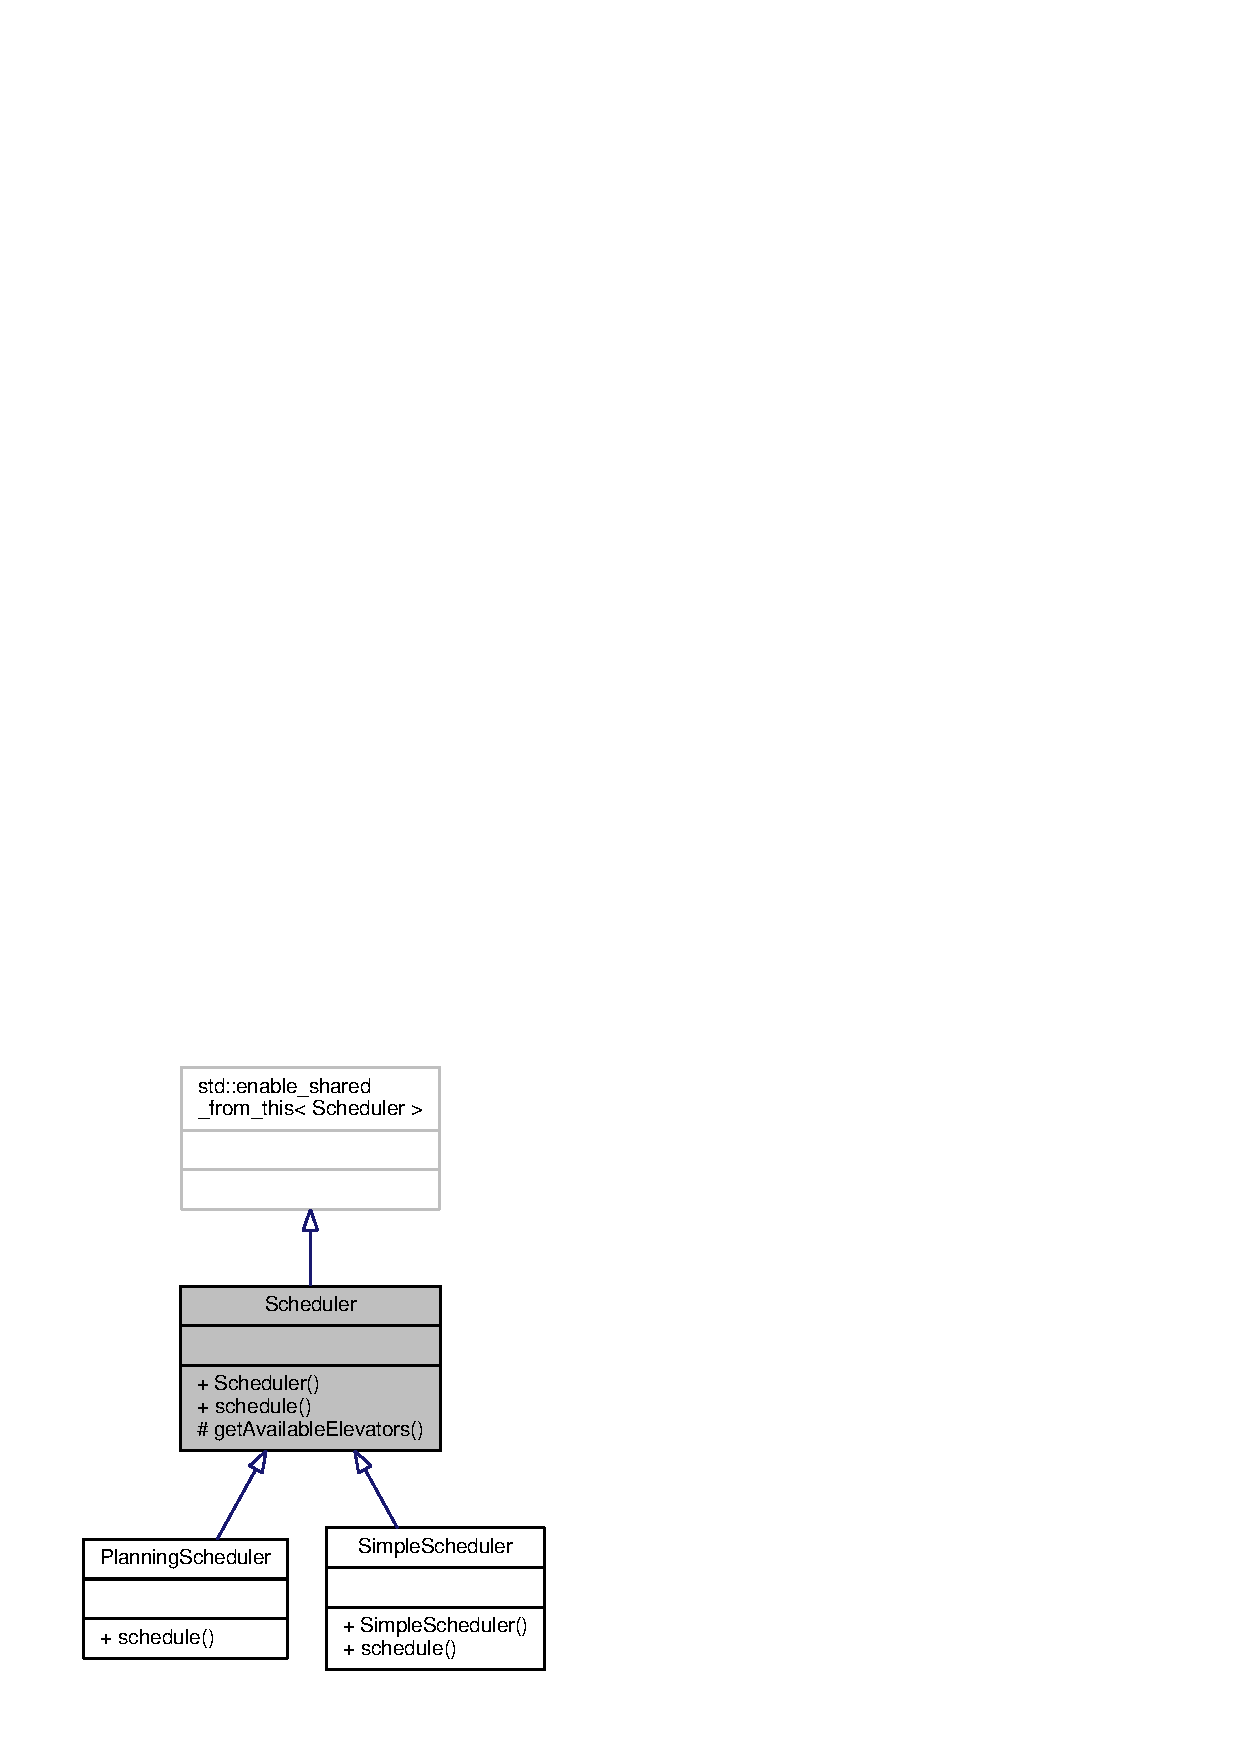
\includegraphics{doc/latex/class_scheduler__inherit__graph}
  \caption{Diagrama UML das classes Scheduler}
  \label{fig:model:schedulers:uml:base}
\end{figure}

Os \textit{schedulers} têm apenas um método público, chamado \textsf{int
  schedule()}, que recebe como parâmetro a função de custo e um ponteiro para o
prédio, além de, opcionalmente, um elevador para ser excluído.

\unsure{Onde falamos de por que é importante excluir elevadores do schedule às
  vezes? (Vanzella)}
Excluir um elevador é importante, como foi falado na Sessão XXX. Há um método
protegido na classe \texttt{Scheduler}, chamado
\texttt{getAvailableElevators()}, que retorna uma lista de elevadores, excluindo
aqueles que não podem ser utilizados.

\subsection{\label{model:schedulers:simple}Simple}
O \textit{Simple Scheduler}, como o nome sugere, tem um comportamento bem
simples: itera pela lista de elevadores disponíveis, calculando a função de
custo para cada um, e retorna o de menor custo.

\subsection{\label{model:schedulers:planning}Planning}
\lipsum[5]

\section{\label{model:costfunctions}Algoritmos de Função de Custo}
\lipsum[5]

\subsection{\label{model:costfunctions:random}Random}
\lipsum[5]

\subsection{\label{model:costfunctions:nn}Nearest Neighbour}
\lipsum[5]

\subsection{\label{model:costfunctions:bnn}Better Nearest Neighbour}
\lipsum[5]

\subsection{\label{model:costfunctions:weighted}Weighted}
\lipsum[5]




% \chapter{\label{chap:modeling}Modelagem do Sistema}

% Um sistema de simulação possui uma série de componentes conceituais, cada um com
% suas responsabilidades bem definidas. Para projetar um simulador, diversas
% abordagens e paradigmas poderiam ser aplicadas. Para o projeto do simulador de
% sistemas de elevadores deste estudo, doravante chamado apenas de simulador,
% optou-se pelo paradigma de \textit{Programação Orientada a Objetos}. Esta
% escolha se deu pelos seguintes motivos:

% \begin{description}
%   \item[Capacidade de Abstração]\hfill \\
%     Conceitos da Programação Orientada a Objetos, como classes, interfaces,
%     polimorfismo, herança e sobrecarga permitem a realização de uma modelagem
%     conceitual em alto nível de abstração, permitindo uma explanação de fácil
%     entendimento sem ser necessário abordar questões da implementação em si
%     (linguagem de programação, arquitetura, etc).
%   \item[Padrão de Mercado]\hfill \\
%     Desde meados dos anos 90, a Programação Orientada a Objetos tornou-se
%     frequentemente utilizada no mercado de desenvolvimento de software e nos
%     ambientes acadêmicos relacionados à computação. Assim, é possível atingir
%     uma maior audiência.
%   \item[Domínio dos Autores]\hfill \\
%     O paradigma é de domínio dos autores deste estudo.
% \end{description}

% Nas próximas seções serão apresentadas as modelagens conceituais para o projeto
% do simulador de elevadores.

% \section{\label{sec:eventos-e-tipos}Eventos e tipos}

% A simulação de eventos discretos, como o próprio nome já diz, é orientada a
% eventos. Isso significa dizer que as alterações no estado do sistema ocorrerão
% somente na ocasião de algum evento e é preciso ser possível representar um
% evento no contexto do simulador.

% Um evento é uma estrutura que deve possuir as seguintes informações: (1) o tipo
% do evento; (2) o horário agendado para a ocorrência do evento; (3) um cliente
% (passageiro) e/ou (4) um elevador e/ou (5) um andar do prédio. As existência de
% informações para os itens (3), (4) e (5) dependem do tipo de evento, que pode
% ser uma das seguintes opções:

% \begin{description}
%   \item[Chegada de grupo de clientes] \hfill \ um grupo de clientes chegou na fila de um andar.
%   \item[Chegada de elevador] \hfill \ um elevador chegou a um andar e abriu as portas.
% \end{description}

% Para o evento \textbf{chegada de um cliente}, é necessário conhecer o cliente e
% o andar. Para o evento \textbf{chegada de um elevator}, é necessário conhecer o
% elevador e o andar. A figura \ref{fig:diagram:event} exibe o diagrama de classes
% para eventos (classe \textit{Event}) e tipos de evento (enumeração
% \textit{EventType}). Adicionalmente foi criada a classe \textit{Config},
% responsável por armazenar informações referentes ao cenário sendo simulado.

% \begin{figure}[htb!]
%   \centering
%   \includegraphics[scale=0.6]{img/Basic.eps}
%   \caption[Diagrama de classes para eventos, tipos e configuração]{Diagrama de classes para eventos, tipos de eventos e configuração da simulação.}
% \label{fig:diagram:event}
% \end{figure}

% \section{\label{sec:reactive}Componentes reativos}

% Durante a execução da simulação, à medida que eventos ocorrem, componentes do
% simulador deverão alterar seu estado interno de acordo com o evento ocorrido,
% levando o estado do simulador a uma nova situação. Estes componentes são:

% \begin{enumerate}
%   \item Relógio da Simulação;
%   \item Estado do Sistema;
%   \item Contadores Estatísticos.
% \end{enumerate}

% A seguir são apresentadas as classes que representam estes componentes no
% simulador.

% \subsection{Estado do sistema}

% Entre os componentes fundamentais de um simulador destaca-se a representação do
% \textit{estado do sistema}, uma coleção de variáveis necessárias para descrever
% o sistema em um instante em particular da simulação \cite{Law}. Neste projeto, a
% classe \textit{Building} é responsável por encapsular o conjunto de informações
% que definem este estado (figura \ref{fig:diagram:model}). Esta classe é
% responsável por gerenciar múltiplas instâncias de elevadores (classe
% \textit{Elevator}), andares (classe \textit{Floor}) e clientes (classe
% \textit{Client}) e relacionar estas instâncias entre si - reproduzindo, deste
% modo, as dinâmicas do sistema do mundo real que está sendo simulado.

% \begin{figure}[htb!]
%   \centering
%   \includegraphics[scale=0.6]{img/Model.eps}
%   \caption{Diagrama de classes do \textit{Estado do Sistema}.}
% \label{fig:diagram:model}
% \end{figure}

% \begin{description}
%   \item[Building] \hfill \\
%     Representa a composição do prédio sendo simulado. Possui um conjunto de
%     elevadores, uma lista ordenada de andares e um método \texttt{reset},
%     utilizado para a inicialização da simulação. Um prédio é formado por no
%     mínimo um elevador e no mínimo um andar\footnote{Isto em termos conceituais;
%     porém, não há sentido na existência de um sistema de elevadores em uma
%     edificação com somente um andar. De fato, conforme afirmado na seção
%     \ref{section:scenarios}, serão simulados prédios com, no mínimo, 4
%     andares.}.

%   \item[Floor] \hfill \\
%     Parte componente de um prédio, possuindo uma numeração e duas
%     filas\footnote{No mundo real, apesar de aparentemente as pessoas formarem
%     uma fila única, os membros da fila respeitam o sentido de viagem do elevador
%     e implicitamente separam-se em duas filas: uma para subir e outra para
%     descer.}: uma para clientes que desejam descer e outra para clientes que
%     desejam subir.

% \item[Elevator] \hfill \\
%     Representa um elevador. Possui como atributos o andar em que se
%     encontra, uma sequência ordenada de andares de destino e um mapa associando
%     andares com conjuntos de clientes - ou seja, para cada andar o mapa reune
%     quais os grupos de clientes que o possuem como destino. Além disso, possui
%     métodos auxiliares para informar o sentido da viagem do elevador
%     (\texttt{direction}), bem como a sua ocupação atual (\texttt{occupation}).

% \item[Client] \hfill \\
%     Representa um grupo de pessoas que desejam utilizar um elevador. Possui como
%     atributos o número de pessoas no grupo (\texttt{partySize}), o horário em
%     que chegou na fila do andar (\texttt{arrivalTime}) e o andar destino para o
%     qual deseja ir (\texttt{destination}).

% \end{description}

% \subsection{Relógio da simulação}

% O \textit{relógio da simulação} é representado pela classe \textit{Timer}
% (figura \ref{fig:diagram:timer}). Esta classe encapsula o acesso ao atributo
% privado \texttt{time}, provendo métodos para inicialização (\texttt{reset}),
% consulta (\texttt{currentTime}), atualização para um valor arbitrário
% (\texttt{advanceTo}) e atualização por incremento (\texttt{advanceBy}).

% \begin{figure}[htb!]
%   \centering
%   \includegraphics[scale=0.6]{img/Timer.eps}
%   \caption{Diagrama de classes do \textit{Relógio da Simulação}.}
% \label{fig:diagram:timer}
% \end{figure}

% \subsection{Contadores estatísticos}

% Os \textit{contadores estatísticos} da simulação são responsáveis por coletar e
% sumarizar dados do sistema durante toda a execução da simulação. Sua existência
% permite a realização de análises qualitativas e quantitativas a respeito do
% sistema simulado.

% Neste projeto, os \textit{contadores estatísticos} são representados pela classe
% \textit{Statistics} (figura \ref{fig:diagram:stats}). Conforme descrito na
% proposta de trabalho deste estudo, o objetivo é encontrar algoritmos que
% otimizem o tempo de espera médio. Porém, armazenar mais dados estatísticos
% permite realizar análises mais ricas, fornecendo informações como desvios, por
% exemplo. Portanto, para cada grupo de clientes transportados pelo sistema serão
% armazenados o seguinte conjunto de informações sobre a viagem (classe
% \textit{Travel}):

% \begin{description}
%   \item[\texttt{origin}] \hfill \\
%     O andar de origem da viagem.

%   \item[\texttt{client}] \hfill \\
%     O grupo de cliente, contendo o tamanho do grupo, a hora em que
%     chegou à fila e o seu andar de destino.

%   \item[\texttt{elevator}] \hfill \\
%     O elevador que transportou o grupo do andar origem ao andar destino, junto
%     de sua ocupação no momento em que parou no andar para o desembarque.

%   \item[\texttt{waitingTime}] \hfill \\
%     O tempo que o grupo esperou na fila - ou seja, o tempo compreendido entre a
%     chegada do grupo na fila e o seu embarque no elevador.

%   \item[\texttt{journeyTime}] \hfill \\
%     O tempo de jornada do grupo - ou seja, o tempo compreendido entre o embarque
%     do grupo no elevador e o desembarque no andar destino.

%   \item[\texttt{arrivalTime}] \hfill \\
%     O horário em que o grupo desembarou no andar destino.
% \end{description}

% Além destes, a classe também possui métodos para inicialização (\texttt{reset})
% e para avaliar se a simulação deve terminar (\texttt{keepRunning})~-~por
% exemplo, o tempo mínimo se simulação já se passou.

% \begin{figure}[htb!]
%   \centering
%   \includegraphics[scale=0.6]{img/Stats.eps}
%   \caption{Diagrama de classes do \textit{Contadores Estatísticos}.}
% \label{fig:diagram:stats}
% \end{figure}

% \section{\label{sec:model:event}Gerenciamento de eventos}

% Na seção \ref{sec:reactive} foram apresentados componentes reativos~-~ou seja,
% que devem reagir na ocorrência de um evento. Porém restam as questões de como
% saber qual evento será o próximo a ocorrer e como notificar os elementos
% reativos disso. Portanto, precisamos de mecanismos para ordenar eventos e
% notificar os componentes da ocorrência de um evento.

% \subsection{Organização e priorização}

% Na seção \ref{simulator:movation:discrete} foi apresentado o \textit{mecanismo de
% avanço de tempo para o próximo evento}, onde deve-se verificar, em uma lista de
% eventos, qual é o próximo evento a ocorrer. Dado um conjunto de eventos
% agendados (ou seja, ainda não ocorridos), o primeiro evento a ocorrer é
% justamente o que possui o menor tempo de agendamento. Um tipo abstrato de dados
% que serve para este propósito é uma \textit{fila prioritária}, ou
% \textit{priority queue}, que funciona de forma similar a filas \textit{FIFO},
% com a diferença de que cada elemento armazenado possui uma prioridade associada.
% A \textit{fila prioritária} irá atender os elementos por ordem de prioridade, da
% maior para a menor. Ao considerar que a prioridade de um evento é inversamente
% proporcional ao instante em que irá ocorrer - ou seja, quanto menor o tempo do
% evento maior é a sua prioridade -, temos uma fila na qual o próximo elemento a
% ser atendido sempre será o próximo evento a ocorrer.

% Assim, a classe \textit{EventQueue} encapsula uma fila prioritária de eventos,
% fornecendo métodos para inserir um evento na fila (\texttt{push}), recuperar e
% remover o próximo evento (\texttt{pop}) ou simplesmente ``espiar'' o próximo
% evento (\texttt{peek}). Juntamente com a classe
% \textit{EventGenerator}\footnote{Classe responsável pela criação de eventos;
% abordada mais adiante neste estudo.}, a \textit{EventQueue} compõe o chamado
% \textit{Sistema de Priorização de Eventos}, ou \textit{SPE}. Assim,
% possibilita-se que facilmente se saiba qual será o próximo evento a ocorrer.

% \begin{figure}[htb!]
%   \centering
%   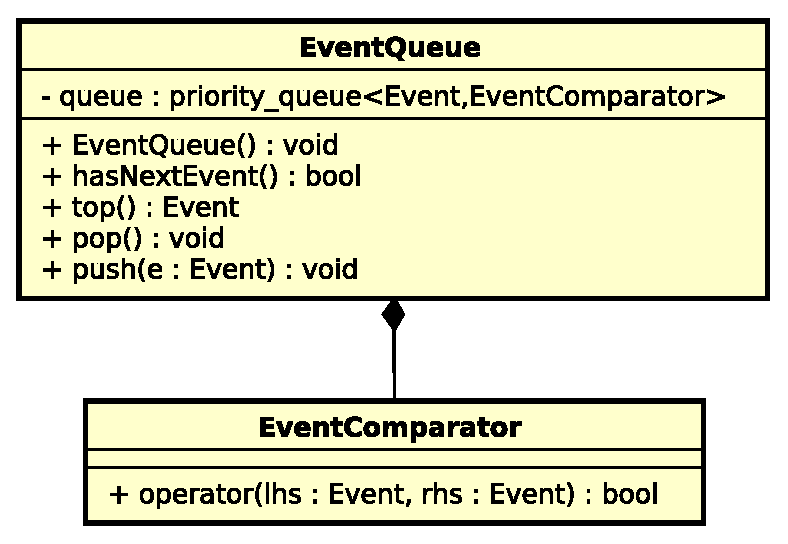
\includegraphics[scale=0.6]{img/EventQueue.eps}
%   \caption{Diagrama de classes do \textit{Sistema de Priorização de Eventos}.}
% \label{fig:diagram:event:manage}
% \end{figure}

% \subsection{\label{sec:model:notify}Notificação}

% Quando o próximo evento a ocorrer é conhecido, o problema passa a ser notificar
% os elementos reativos que este evento ocorreu para que os mesmos possam
% atualizar seus estados internos. De acordo com Gamma
% \cite{Gamma:1995:DPE:186897}, o padrão \textit{Observer} é um \textit{design
% pattern} indicado para resolver este problema. Este \textit{pattern} define uma
% dependência de um-para-muitos ($1:N$) entre objetos de modo que, quando este um
% objeto (\textit{subject}) tem seu estado alterado, todos os seus dependentes
% (\textit{observers}) são notificados deste mudança. Por consequência, estes
% dependentes podem modificar seu estado interno baseando-se nas informações desta
% notificação. Neste projeto, o subsistema que segue o \textit{Observer pattern}
% será chamado de \textit{Sistema de Notificação de Eventos}, ou \textit{SNE}.

% Os três principais componentes do \textit{SNE} (figura
% \ref{fig:diagram:notification}) são duas interfaces e uma classe:

% \begin{description}
%   \item[EventObserver] \hfill \\
%     Interface a ser realizada por qualquer classe que deseje receber
%     notificações de eventos. Seu único método, \texttt{notify}, permite o
%     recebimento de uma notificação de um evento.

%   \item[EventNotifier] \hfill \\
%     Interface a ser realizada por qualquer classe que deseje notificar a
%     ocorrência de eventos. Define métodos que objetos que implementem a
%     interface \textit{EventObserver} possam registrar (\texttt{register}) ou
%     desregistrar (\texttt{unregister}) para receber notificações de ocorrências
%     de um determinado tipo de evento, além do método \texttt{notify}, que deverá
%     notificar um evento para todos os \textit{observers} registrados.

% \item[EventDispatcher] \hfill \\
%     Classe concreta que realiza a interface \textit{EventNotifier}. Deve possuir
%     uma estrutura de dados para armazenar quais \textit{observers} se
%     registraram para cada tipo de evento. Na ocorrência de um evento, o
%     \textit{EventDispatcher} é responsável por varrer a lista de
%     \textit{observers} registrados e notificá-los de acordo com o tipo de evento
%     ocorrido.

% \end{description}

% \begin{figure}[htb!]
%   \centering
%   \includegraphics[scale=0.6]{img/Notification.eps}
%   \caption{Diagrama de classes do \textit{Sistema de Notificação de Eventos}.}
% \label{fig:diagram:notification}
% \end{figure}

% Três importantes componentes do simulador podem se beneficiar desta construção:
% (1) o \textit{relógio do sistema} (classe \textit{Timer}); (2) os
% \textit{contadores estatísticos} (classe \textit{Statistics}); e (3) o
% \textit{estado do sistema} (classe \textit{Building}). Na ocorrência de um
% evento, estas três entidades devem ser notificadas e cada uma irá alterar seu
% estado interno da forma adequada. Para isto, devem implementar a interface
% \textit{EventObserver} e registrarem-se no \textit{EventDispatcher}, conforme
% ilustrado na figura \ref{fig:diagram:observers}. Assim, o
% \textit{EventDispatcher} e a \textit{EventQueue} podem, juntos, notificar aos
% componentes reativos exatamente qual evento ocorreu em cada iteração da
% simulação, na ordem correta dos eventos.

% \begin{figure}[htb!]
%   \centering
%   \includegraphics[scale=0.6]{img/Observers.eps}
%   \caption{Diagrama de classes dos \textit{observers}.}
% \label{fig:diagram:observers}
% \end{figure}

% \section{\label{sec:model:generator}Criação}

% Como foi mostrado na seção~\ref{sec:eventos-e-tipos}, há dois eventos onde há
% alteração no \textit{estado do sistema}: \textbf{chegada de passageiros} e
% \textbf{chegada de elevador a um andar}.

% A chegada de um elevador é um evento determinístico~-~sabe-se que o elevador
% viaja a uma velocidade constante e conhece-se sua agenda interna. Portanto o
% tempo entre um elevador sair de um andar e o evento deste chegar a outro andar é
% fixo. Isto é, para um elevador que leva $t$ segundos para se deslocar um andar,
% após sair de um andar $a_{0}$ no tempo $t_{0}$ e subir ou descer $a$ andares, o evento
% de chegar ao andar $a_{0} + a$ ocorrerá no tempo $t_{0} + at$.

% Já a chegada de passageiros segue modelos estocásticos, descritos na seção~\ref{chap:input}.

% A figura~\ref{fig:diagram:generator} mostra o diagrama UML da classe que gera eventos.

% \begin{figure}[htb!]
%   \centering
%   \includegraphics[scale=0.6]{img/EventGenerator.eps}
%   \caption{Diagrama de classes do \textit{Sistema de Geração de Eventos}.}
% \label{fig:diagram:generator}
% \end{figure}

% \subsection{\label{chap:input}Entrada de distribuição de probabilidade}

% Segundo~\cite{Ross:2006:IPM:1197141}, a taxa de chegada de clientes é um
% processo de Poisson, com razão $\lambda$. Ou seja, o tempo entre novos clientes
% são variáveis exponenciais independentes, com valor esperado
% $\frac{1}{\lambda}$. Esta distribuição varia de acordo com a hora do dia. Por
% exemplo, nos horários do início do turno da manhã e no início do turno da tarde,
% muito mais passageiros chegam ao térreo, com destino ao andar onde trabalham.

% A distribuição de Poisson é dada na seguinte forma:

% \[f(k,\lambda) = \frac{\lambda^{k}e^{-k}}{k!}\]

% onde $\lambda$ é o valor esperado e a variância e $k$ é um inteiro não-negativo que, no caso
% deste sistema, representa um momento do dia.

% Pode-se ver na figura~\ref{fig:distribution:poisson} um exemplo de diferentes
% valores de $\lambda$ gerando diferentes distribuições.

% \begin{figure}[htb!]
%   \centering
%   \includegraphics[scale=1.0]{img/poisson.eps}
%   \caption{Exemplo de distribuições de Poisson.}
% \label{fig:distribution:poisson}
% \end{figure}

% Já a probabilidade de um cliente ir de um andar para outro, em um tráfego
% chamado de \textit{interfloor}, é um processo de Markov, com distribuições
% normais que variam de acordo com a hora do dia.

% Uma cadeia de Markov, utilizada para representar este processo, é por sua vez
% representada por uma matriz de probabilidades. No caso deste sistema, tem-se uma
% função com distribuição normal (\textit{i.e.} uma média e um desvio padrão) que
% varia de acordo com o horário do dia, para cada posição desta matriz.

% Um exemplo de matriz para um prédio de 3 andares é:

% \[
%   \begin{bmatrix}
%     f_{11} & f_{12} & f_{13} \\
%     f_{21} & f_{22} & f_{23} \\
%     f_{31} & f_{32} & f_{33}
%   \end{bmatrix}
% \]

% Onde cada valor é uma função $f(t)$, com $t$ sendo o momento do dia e resultando
% em um valor de média e um valor de desvio padrão para a distribuição naquele
% momento. Cada função descreve a probabilidade de um cliente estar em um andar e
% desejar ir para outro. Por exemplo, $f_{31}$ descreve a probabilidade de um
% cliente estar no terceiro andar e desejar descer para o primeiro.

% Além disto, a diagonal principal (\textit{i.e} $f_{11}$, $f_{22}$ e
% $f_{33}$) é sempre zero, já que não faz sentido um cliente desejar ir para o
% mesmo andar em que se encontra.

% Esta cadeia de Markov pode ser vista na figura~\ref{fig:distribution:markov}.

% \begin{figure}[htb!]
%   \centering
%   \includegraphics[scale=0.6]{img/markov.eps}
%   \caption{Exemplo de cadeia de Markov para um prédio de 3 andares.}
% \label{fig:distribution:markov}
% \end{figure}

% \section{\label{sec:model:report}Geração de relatórios}

% Por último mas não menos importante, é apresentada a classe
% \textit{ReportBuilder}, ilustrado pela figura \ref{fig:diagram:report}. Esta
% classe tem por responsabilidade a elaboração de um relatório (em arquivo) a
% partir da configuração da simulação e das estatísticas acumuladas durante a
% execução.

% \begin{figure}[htb!]
%   \centering
%   \includegraphics[scale=0.6]{img/Report.eps}
%   \caption{Diagrama de classes do \textit{ReportBuilder}.}
% \label{fig:diagram:report}
% \end{figure}

% \subsection{Exemplo de relatório}
% Com base nas informações estatísticas, pretende-se a obtenção de um relatório
% sumarizando e detalhando diversas informações com aproximadamente o
% \textit{layout} a seguir:

% \begin{lstlisting}
% Título:       Prédio comercial de tamanho médio
% Andares:      99
% Elevadores:   99
% Carga máxima: 99
% Algoritmo:    Planning (horizonte 9)
% ---------------------------------------------------------
% Período simulado: 99 horas
% Horário inicial:  00:00:00
% Horário final:    23:59:59
% ---------------------------------------------------------
% Passageiros transportados: 9999
% Total de paradas: 999

%        Total    Média   Desvio
% AWT    99999    99999    99999
% AJT    99999    99999    99999
% ---------------------------------------------------------
%               Tempo em  Tempo     Total         Ocupação
%               viagem    Ocioso    Passageiros   Média
% Elevador 1    99%       99%       999           99%
% Elevador 2    99%       99%       999           99%
% Elevador 3    99%       99%       999           99%
% ...
% Elevador 99   99%       99%       999           99%
% ---------------------------------------------------------
% Simulação executada em 99:99:99.
% \end{lstlisting}

% \section{Simulador completo}

% O uso de instâncias de todas estas classes juntas dá forma ao simulador,
% conforme proposto por \cite{Law,Banks}. O componente responsável por orquestrar
% as interações entre estas instâncias e garantir o fluxo de execução é
% representado pela classe \textit{Simulator}.

% Esta classe não possui atributos ou métodos específicos; somente as instâncias
% das outras classes e um método que realiza um laço indefinido, onde um evento é
% recuperado e notificado para os componentes reativos; estes, por sua vez,
% atualizam seu estado interno e agendam novos eventos; a simulação segue até que
% a condição de parada seja satisfeita. O algoritmo \ref{alg:sim} mostra um
% pseudo-código de como poderia ser este método de execução da simulação.

% \begin{figure}[htb!]
%   \centering
%   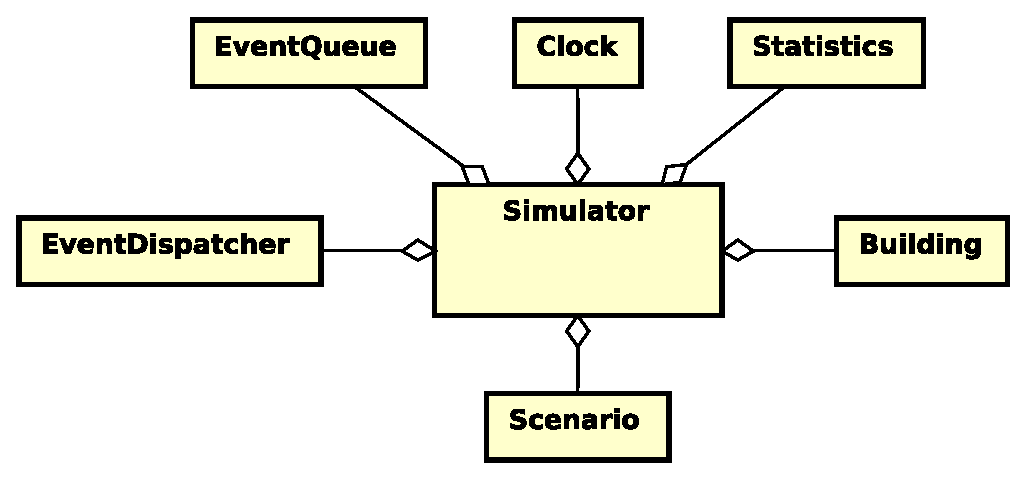
\includegraphics[scale=0.6]{img/Simulator.eps}
%   \caption{Diagrama de classes do simulador}
% \label{fig:diagram:simulator}
% \end{figure}

% \begin{algorithm}[H]
% \begin{center}
% \begin{algorithmic}[1]
% \Function{run}{$config, timer, statistics, building, dispatcher, eventQueue, reportBuilder$}
%   \State $timer.$\Call{Reset}{$config$}
%   \State $statistics.$\Call{Reset}{$config$}
%   \State $building.$\Call{Reset}{$config$}
%   \State $dispatcher.$\Call{Register}{$EventType.Any, timer$}
%   \State $dispatcher.$\Call{Register}{$EventType.Any, statistics$}
%   \State $dispatcher.$\Call{Register}{$EventType.Any, building$}
%   \While{$statistics.$\Call{KeepRunning}{}}
%     \State $nextEvent \gets eventQueue.$\Call{Pop}{}
%     \State $dispatcher.$\Call{Notify}{$nextEvent$}
%   \EndWhile
%   \State $reportBuilder.$\Call{BuildReport}{$config, statistics$}
% \EndFunction
% \end{algorithmic}
% \end{center}
% \caption
%    {\label{alg:sim}Algoritmo de simulação.}
% \end{algorithm}

\chapter{\label{chap:results}Resultados}

\section{Cenário \textit{Low-rise}}

\lipsum[1]

\begin{table}[htb!]
\centering
\caption{Parâmetros do cenário \textit{Low-rise}.}
\label{tab:results:lowrise:params}
\begin{tabular}{|r|l|}
\hline
\textbf{Propriedade}          & \textbf{Valor}       \\ \hline
\textit{Nome}                 & Low-rise             \\ \hline
\textit{Duração (s)}          & 43200                \\ \hline
\textit{Semente}              & 54TH7hboAG1iOsDIDhJp \\ \hline
\textit{Elevatores}           & 2                    \\ \hline
\textit{Capacidade}           & 6                    \\ \hline
\textit{Andares}              & 11                   \\ \hline
\textit{Horizonte (planning)} & 5                    \\ \hline
\end{tabular}
\end{table}

\begin{table}[htb!]
\centering
\caption{Resultados obtidos da simulação do cenário \textit{Low-rise}.}
\label{tab:results:lowrise}
\begin{tabular}{|l|r|r|r|r|r|r|}
\hline
\multicolumn{1}{|c|}{\textbf{}}                 & \multicolumn{3}{c|}{\textbf{Tempo de Espera}}                                                                    & \multicolumn{3}{c|}{\textbf{Tempo de Jornada}}                                                                                                                       \\ \hline
\textbf{Estratégia} & \multicolumn{1}{c|}{\textit{Médio}} & \multicolumn{1}{c|}{\textit{Desvio}} & \multicolumn{1}{c|}{\textit{Total}} & \multicolumn{1}{c|}{\textit{Médio}}                   & \multicolumn{1}{c|}{\textit{Desvio}}                  & \multicolumn{1}{c|}{\textit{Total}}                  \\ \hline
\textit{Simple / Random}          & \cellcolor[HTML]{FD6864}5.4064      & \cellcolor[HTML]{FD6864}4.1792       & \cellcolor[HTML]{FD6864}16933       & \cellcolor[HTML]{FD6864}{\color[HTML]{000000} 4.4949} & 2.8676                                                & \cellcolor[HTML]{FD6864}{\color[HTML]{000000} 14078} \\ \hline
\textit{Planning / Random}        & \cellcolor[HTML]{67FD9A}3.1580      & \cellcolor[HTML]{67FD9A}2.8688       & \cellcolor[HTML]{67FD9A}9891        & 4.4713                                                & \cellcolor[HTML]{FD6864}{\color[HTML]{000000} 3.0005} & 14004                                                \\ \hline
\textit{Simple / NN}              & 3.5144                              & \cellcolor[HTML]{FFFFFF}3.5768       & 11007                               & 4.4700                                                & 2.8565                                                & 14000                                                \\ \hline
\textit{Planning / NN}            & 3.2273                              & 3.0515                               & 10108                               & 4.4770                                                & 2.9796                                                & 14022                                                \\ \hline
\textit{Simple / BNN}             & 3.3547                              & 3.2931                               & 10507                               & 4.4674                                                & 2.9163                                                & 13992                                                \\ \hline
\textit{Planning / BNN}           & 3.1830                              & 2.9150                               & 9969                                & \cellcolor[HTML]{67FD9A}4.4623                        & \cellcolor[HTML]{FFFFFF}2.9787                        & \cellcolor[HTML]{67FD9A}13976                        \\ \hline
\textit{Simple / Weighted}        & 3.7149                              & 3.8036                               & 11635                               & 4.4719                                                & \cellcolor[HTML]{67FD9A}2.7997                        & 14006                                                \\ \hline
\textit{Planning / Weighted}      & 3.2529                              & 3.0760                               & 10188                               & 4.4789                                                & 2.9714                                                & 14028                                                \\ \hline
\end{tabular}
\end{table}

\begin{figure}[htb]
  \centering
  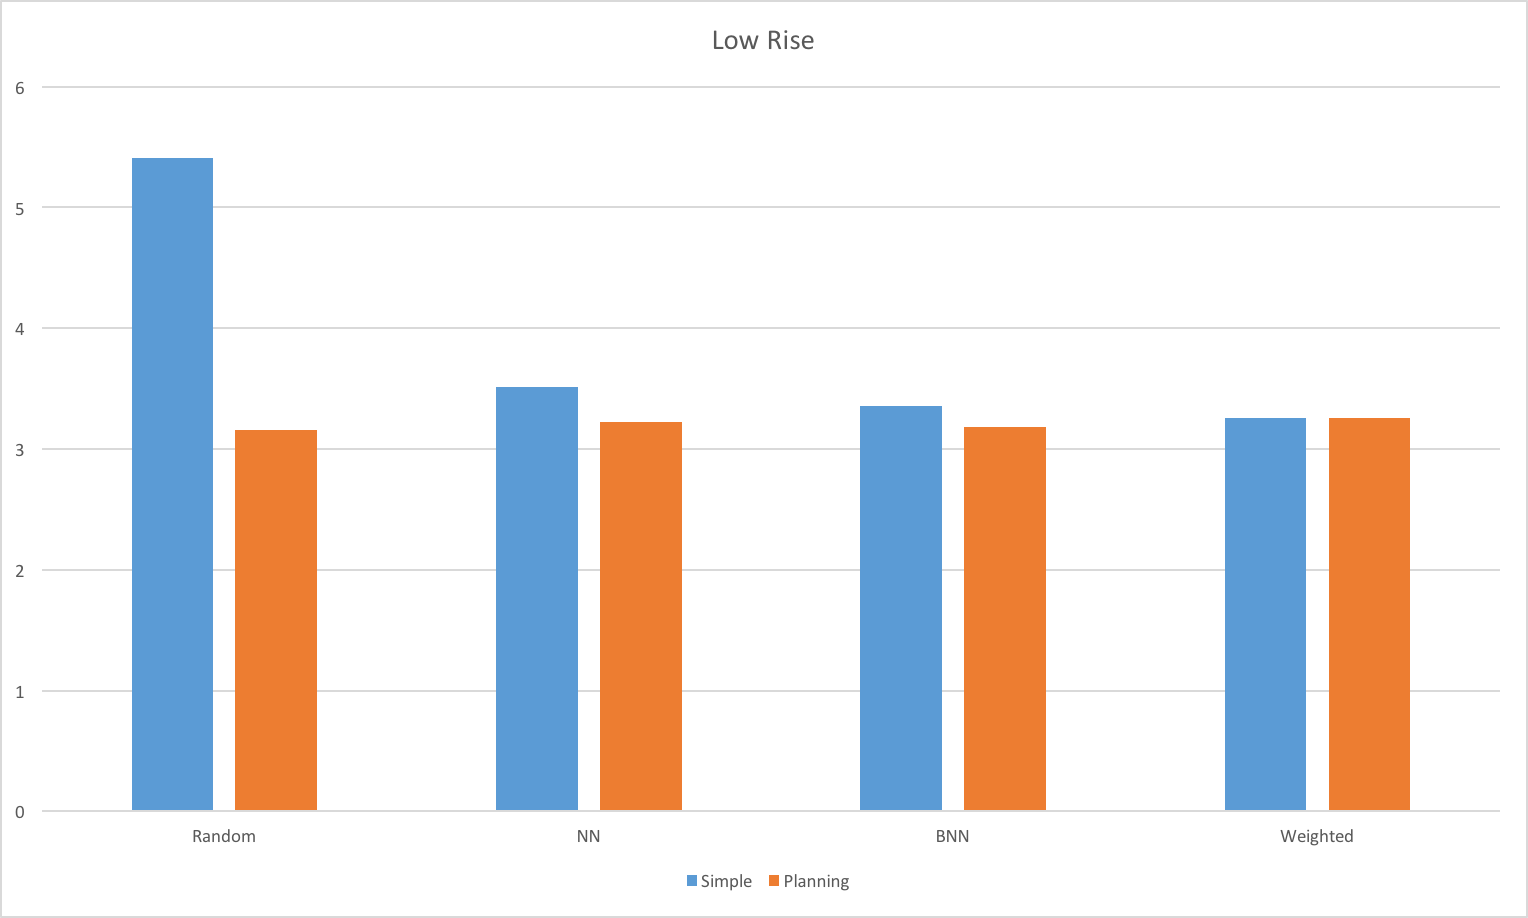
\includegraphics[scale=0.5]{img/chart-averages-low-rise}
  \caption{Comparação do tempo médio de espera com as diferentes estratégias
    para o cenário \textit{Low Rise}}
  \label{fig:result:average:low-rise}
\end{figure}

\section{Cenário \textit{High-rise}}

\lipsum[1]

\begin{table}[htb!]
\centering
\caption{Parâmetros do cenário \textit{High-rise}.}
\label{tab:results:highrise:params}
\begin{tabular}{|r|l|}
\hline
\textbf{Propriedade}          & \textbf{Valor}       \\ \hline
\textit{Nome}                 & High-rise            \\ \hline
\textit{Duração (s)}          & 43200                \\ \hline
\textit{Semente}              & w9JwgykwejtoL2icSgHo \\ \hline
\textit{Elevatores}           & 8                    \\ \hline
\textit{Capacidade}           & 10                   \\ \hline
\textit{Andares}              & 39                   \\ \hline
\textit{Horizonte (planning)} & 2                    \\ \hline
\end{tabular}
\end{table}

\begin{table}[htb!]
\centering
\caption{Resultados obtidos da simulação do cenário \textit{High-rise}.}
\label{tab:results:highrise}
\begin{tabular}{|l|r|r|r|r|r|r|}
\hline
\multicolumn{1}{|c|}{\textbf{}}                 & \multicolumn{3}{c|}{\textbf{Tempo de Espera}}                                                                    & \multicolumn{3}{c|}{\textbf{Tempo de Jornada}}                                                                                                                       \\ \hline
\textbf{Estratégia} & \multicolumn{1}{c|}{\textit{Médio}} & \multicolumn{1}{c|}{\textit{Desvio}} & \multicolumn{1}{c|}{\textit{Total}} & \multicolumn{1}{c|}{\textit{Médio}}                   & \multicolumn{1}{c|}{\textit{Desvio}}                  & \multicolumn{1}{c|}{\textit{Total}}                  \\ \hline
\textit{Simple / Random}          & 25.9981                         & 28.0464                         & 190124                          & \cellcolor[HTML]{FD6864}15.2595 & 14.9190                         & \cellcolor[HTML]{FD6864}111593  \\ \hline
\textit{Planning / Random}        &  8.8829                         & 16.5500                         &  64961                          & 15.1742                         & 12.0139                         & 110969                          \\ \hline
\textit{Simple / NN}              & 20.3395                         & 37.1902                         & 148743                          & 15.0993                         & 11.4479                         & 110421                          \\ \hline
\textit{Planning / NN}            &  9.9824                         & 19.4451                         &  73001                          & 15.1991                         & 11.4878                         & 111151                          \\ \hline
\textit{Simple / BNN}             & 13.5243                         & 23.5950                         &  98903                          & 15.0550                         & \cellcolor[HTML]{67FD9A}10.2476 & 110097                          \\ \hline
\textit{Planning / BNN}           & \cellcolor[HTML]{67FD9A}8.8202  & \cellcolor[HTML]{67FD9A}16.1712 & \cellcolor[HTML]{67FD9A} 64502  & 15.0982                         & 11.9491                         & 110413                          \\ \hline
\textit{Simple / Weighted}        & \cellcolor[HTML]{FD6864}31.0373 & \cellcolor[HTML]{FD6864}54.5909 & \cellcolor[HTML]{FD6864}226976  & \cellcolor[HTML]{67FD9A}14.9915 & \cellcolor[HTML]{FD6864}18.9700 & \cellcolor[HTML]{67FD9A}109633  \\ \hline
\textit{Planning / Weighted}      & 11.3271                         & 22.3406                         &  82835                          & 15.1173                         & 10.8752                         & 110553                          \\ \hline
\end{tabular}
\end{table}

\begin{figure}[htb]
  \centering
  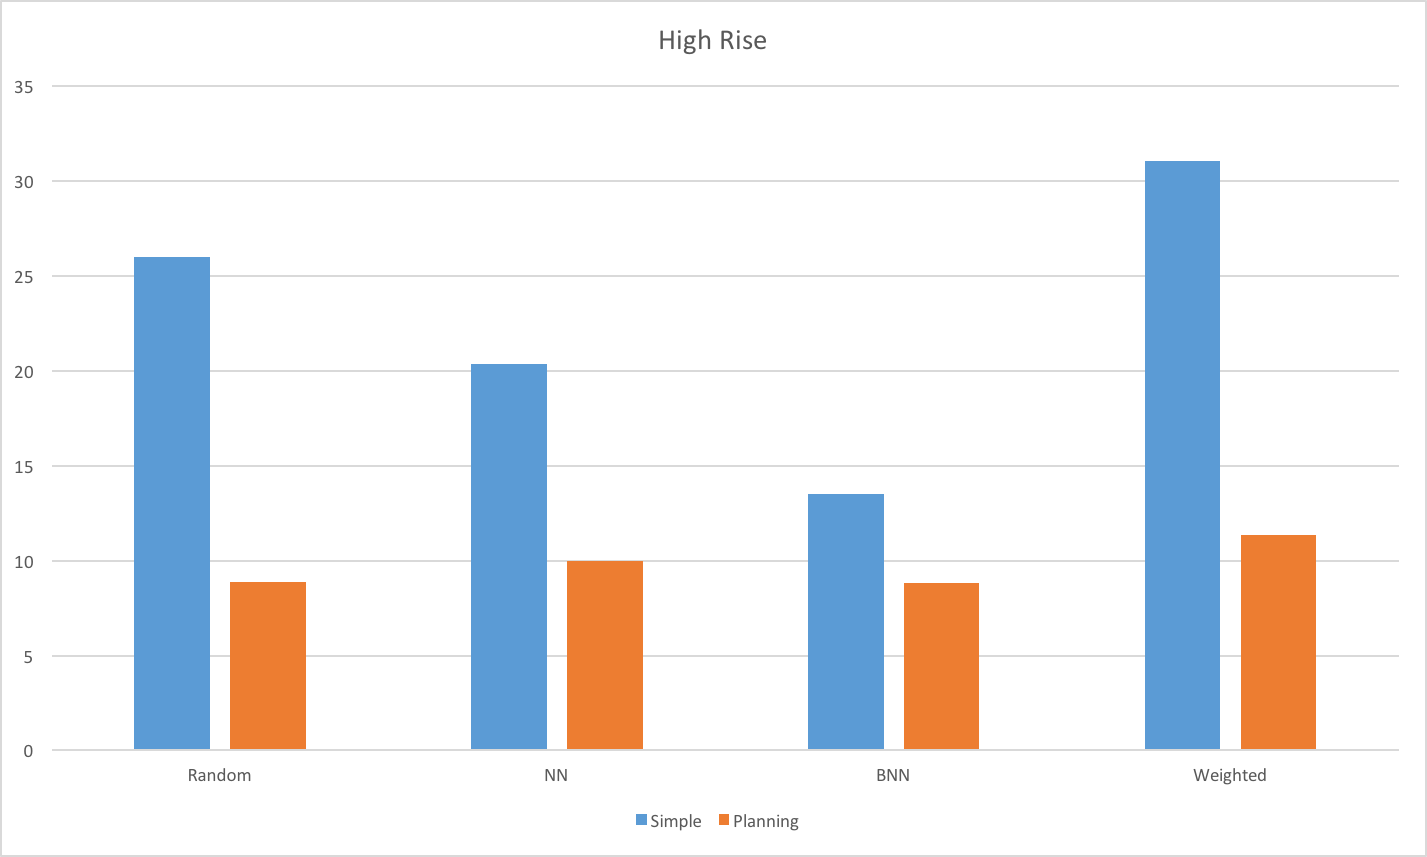
\includegraphics[scale=0.5]{img/chart-averages-high-rise}
  \caption{Comparação do tempo médio de espera com as diferentes estratégias
    para o cenário \textit{High Rise}}
  \label{fig:result:average:high-rise}
\end{figure}

\section{Cenário \textit{Skyscraper}}

\lipsum[1]

\begin{table}[htb!]
\centering
\caption{Parâmetros do cenário \textit{Skyscraper}.}
\label{tab:results:skyscraper:params}
\begin{tabular}{|r|l|}
\hline
\textbf{Propriedade}          & \textbf{Valor}       \\ \hline
\textit{Nome}                 & Skyscraper           \\ \hline
\textit{Duração (s)}          & 43200                \\ \hline
\textit{Semente}              & NimatYvEnU9QeE3GkF4J \\ \hline
\textit{Elevatores}           & 16                   \\ \hline
\textit{Capacidade}           & 12                   \\ \hline
\textit{Andares}              & 163                  \\ \hline
\textit{Horizonte (planning)} & 2                    \\ \hline
\end{tabular}
\end{table}

\begin{table}[htb!]
\centering
\caption{Resultados obtidos da simulação do cenário \textit{Skyscraper}.}
\label{tab:results:skyscraper}
\begin{tabular}{|l|r|r|r|r|r|r|}
\hline
\multicolumn{1}{|c|}{\textbf{}}                 & \multicolumn{3}{c|}{\textbf{Tempo de Espera}}                                                                    & \multicolumn{3}{c|}{\textbf{Tempo de Jornada}}                                                                                                                       \\ \hline
\textbf{Estratégia} & \multicolumn{1}{c|}{\textit{Médio}} & \multicolumn{1}{c|}{\textit{Desvio}} & \multicolumn{1}{c|}{\textit{Total}} & \multicolumn{1}{c|}{\textit{Médio}}                   & \multicolumn{1}{c|}{\textit{Desvio}}                  & \multicolumn{1}{c|}{\textit{Total}}                  \\ \hline
\textit{Simple / Random}          & \cellcolor[HTML]{FD6864}442.2165  & \cellcolor[HTML]{FD6864}1775.3156   & \cellcolor[HTML]{FD6864}10538904  & 54.7816                         & \cellcolor[HTML]{FD6864}389.3520  & 1305554                         \\ \hline
\textit{Planning / Random}        & \cellcolor[HTML]{67FD9A}74.9480   & \cellcolor[HTML]{67FD9A}198.3020    & \cellcolor[HTML]{67FD9A}1786161   & \cellcolor[HTML]{FD6864}59.1500 & \cellcolor[HTML]{67FD9A}46.7326   & \cellcolor[HTML]{FD6864}1409662 \\ \hline
\textit{Simple / NN}              & 343.5988                          & 1426.3821                           &  8188647                          & 54.9789                         & 291.2258                          & 1310258                         \\ \hline
\textit{Planning / NN}            & 103.6866                          &  307.8567                           &  2471058                          & 57.5756                         &  62.5268                          & 1372142                         \\ \hline
\textit{Simple / BNN}             & 287.1803                          & 1137.2342                           &  6844080                          & 55.0124                         & 235.4007                          & 1311056                         \\ \hline
\textit{Planning / BNN}           &  87.0986                          &  239.3584                           &  2075733                          & 58.2380                         &  51.9262                          & 1387928                         \\ \hline
\textit{Simple / Weighted}        & 293.8791                          & 1018.5118                           &  7003726                          & \cellcolor[HTML]{67FD9A}54.6163 & 242.3278                          & \cellcolor[HTML]{67FD9A}1301616 \\ \hline
\textit{Planning / Weighted}      &  99.2689                          &  314.6784                           &  2365776                          & 57.4469                         &  59.3754                          & 1369074                         \\ \hline
\end{tabular}
\end{table}

\begin{figure}[htb]
  \centering
  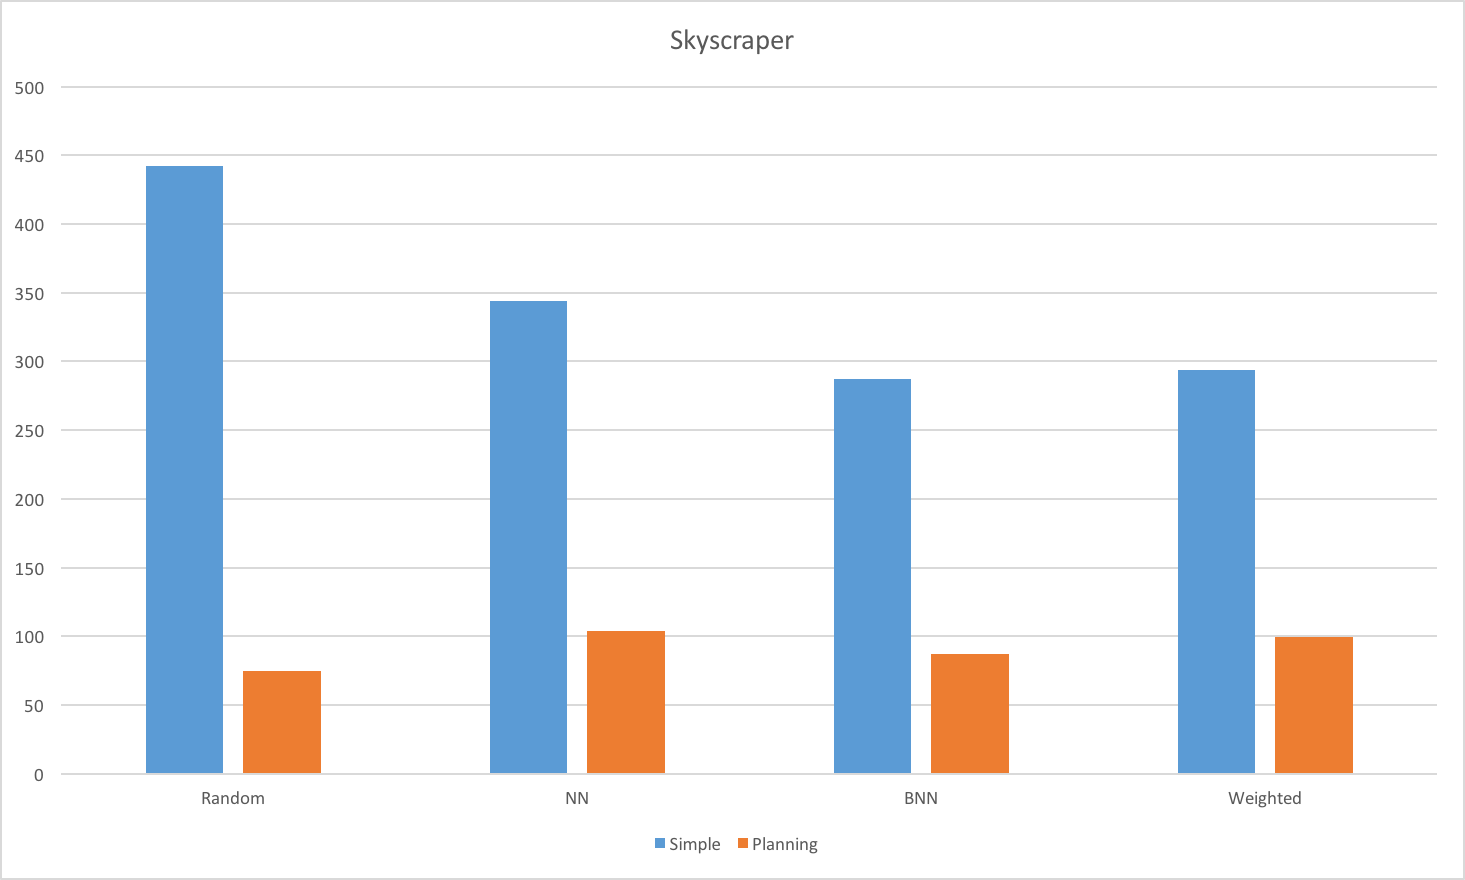
\includegraphics[scale=0.5]{img/chart-averages-skyscraper}
  \caption{Comparação do tempo médio de espera com as diferentes estratégias
    para o cenário \textit{Skyscraper}}
  \label{fig:result:average:skyscraper}
\end{figure}
\chapter{\label{chap:conclusion}Conclusão}

Sendo os elevadores um meio de transporte presente na vida cotidiana de tantos
habitantes de grandes centros urbanos, eles são um alvo para otimização. Porém,
ao contrário do que acreditava-se antes da realização deste trabalho, encontrar
uma solução para este problema está longe do trivial. Nas últimas décadas,
diversas linhas de pesquisa científica~-~dentro e fora da indústria e de seus
segredos industriais e patentes~-~buscaram evoluir os sistemas de elevadores e a
forma com que seus usuários os utilizam.

Um simulador que permita a avaliação objetiva e comparação de diferentes
estratégias em diferentes cenários foi de grande valor, e espera-se que continue
se mostrando de valor também para pesquisas futuras e para o próprio mercado de
fabricantes de elevadores. Isto por que o simulador é uma plataforma de
validação de estratégias~-~e não só as estratégias implementadas durante o tempo
limitado dedicado para este estudo mas também como qualquer estratégia que venha
a ser implementada no futuro.

Notou-se que estratégias que consideram mais dados~-~como a ocupação do
elevador~-~muitas vezes geram resultados melhores com um baixo custo
computacional. Ainda que o ganho seja pequeno, o custo de implementação é,
muitas vezes, essencialmente nulo.

A estratégia de \textit{Planning} se mostrou muito vantajosa, principalmente
conforme o tamanho do prédio aumenta. No entanto, o processamento necessário
para realizá-la é bastante grande, e o custo de implementação em sistemas reais
pode se provar proibitivo. Além disto, o custo computacional cresce bastante
conforme o número de andares e de elevadores aumenta. Horizontes maiores que $2$
se mostraram proibitivamente caros, em tempo de execução, para prédios com mais
de $100$ andares. Mesmo para prédios menores, com até $20$ andares, horizontes
maiores que $5$ não são viáveis. No entanto, isto não é um problema tão grande,
pois
\unsure{Law of diminishing returns. Como exmplico isso? Cada vez ganhamos
  ``menos a mais''. (Vanzella)}

\section{Trabalhos Futuros}

A literatura sugere que algumas técnicas não são vantajosas. Por exemplo, o uso
de algoritmos genéticos~\cite{KOEHLEROTTIGER02} para a definição de zonas de
atuação não é uma boa solução, bem como todas as outras que forçam o usuário a
descobrir qual carro atenderá seu chamado. O mesmo artigo mostra que o sistema
de controle de destino~\cite{KOEHLEROTTIGER02} obtém bons resultados, mas também
sofre do problema de onerar o usuário.

Já os artigos vistos trouxeram algumas das soluções mais promissoras: o
primeiro, a utilização de lógica~\textit{fuzzy} para reconhecimento de padrões
de tráfego e ajuste dinâmico do comportamento dos carros~\cite{marja97}; o
segundo, propondo um modelo estatístico~\cite{DBLP:journals/corr/abs-1212-2499}
que resultou em uma métrica para sucesso: o tempo de espera do usuário sendo
reduzido de 5\% a 55\% em comparação com o algoritmo
trivial~\cite{DBLP:journals/corr/abs-1212-2499}.

Trabalhos futuros podem analizar estas sugestões, utilizando-se do
\textit{framework} construído neste trabalho. Outras políticas mais simples
também podem ser avaliadas, implementando novas funções de custo que levam em
consideração mais dados.

Há também uma gama de políticas de ociosidade dos
elevadores\footnote{\textit{i.e.}, o que fazer quando o elevador está
  parado~-~deixá-lo no mesmo lugar, ou levá-lo para algum outro? Como tomar esta
decisão?}, que pode ser testada em combinação com as políticas de escolha de elevador.

Simulações mais ricas podem ser obtidas variando as distribuições de
probabilidade de chegada e saída nos andares. Por exemplo, variando os
parâmetros com o tempo, para fazer mais clientes chegarem no lobby pela manhã ou
simular um prédio onde há muito tráfego entre um par de andares durante algumas
horas do dia.

Trabalhos mais simples, mas não por isso menos interessantes, podem avaliar o
impacto da escolha do número de elevadores para um determinado prédio, ou ainda
o impacto de políticas de exclusão de atendimento por alguns elevadores a alguns
andares~-~\textit{i.e.} um elevador que só atende certos andares.

Há, sem dúvida, muitas opções para trabalhos futuros que utilizem o conhecimento
construído neste trabalho, e que poderão gerar valor real, tanto acadêmico
quanto para a indústria.


\bibliographystyle{tcc-num}
\bibliography{bib-proposta}

\end{document}
